%============================================================================
% tento soubor pouzijte jako zaklad
% (c) 2008 Michal Bidlo
% E-mail: bidlom AT fit vutbr cz
%============================================================================
% kodovaní: iso-8859-2 (zmena prikazem iconv, recode nebo cstocs)
%----------------------------------------------------------------------------
% zpracování: make, make pdf, make desky, make clean
% připomínky posílejte na e-mail: bidlom AT fit.vutbr.cz
%============================================================================
%\documentclass[cover]{fitthesis} % odevzdani do wisu - odkazy, na ktere se da klikat
%\documentclass[cover,print]{fitthesis} % pro tisk - na odkazy se neda klikat
%\documentclass[english,print]{fitthesis} % pro tisk - na odkazy se neda klikat
\documentclass[cover,english]{fitthesis}
% * Je-li prace psana v anglickem jazyce, je zapotrebi u tridy pouzit 
%   parametr english nasledovne:
%      \documentclass[english]{fitthesis}
% * Neprejete-li si vysazet na prvni strane dokumentu desky, zruste 
%   parametr cover

% zde zvolime kodovani, ve kterem je napsan text prace
% "latin2" pro iso8859-2 nebo "cp1250" pro windows-1250, "utf8" pro "utf-8"
%\usepackage{ucs}
\usepackage[utf8]{inputenc}
\usepackage[T1, IL2]{fontenc}
\usepackage{url}
\DeclareUrlCommand\url{\def\UrlLeft{<}\def\UrlRight{>} \urlstyle{tt}}

%zde muzeme vlozit vlastni balicky

\usepackage{amsthm}
\usepackage{amsfonts}
\usepackage{amsmath}
\usepackage{mdwlist}
\usepackage{textcomp}
\usepackage{verbatim}
\usepackage{tikz}
\usepackage[longend,ruled,vlined,commentsnumbered,linesnumbered,czech]{algorithm2e}

\newtheorem{definition}{Definition}[section]

% =======================================================================
% balíček "hyperref" vytváří klikací odkazy v pdf, pokud tedy použijeme pdflatex
% problém je, že balíček hyperref musí být uveden jako poslední, takže nemůže
% být v šabloně
\ifWis
\ifx\pdfoutput\undefined % nejedeme pod pdflatexem
\else
  \usepackage{color}
  %\usepackage[unicode,colorlinks,hyperindex,plainpages=false,pdftex]{hyperref}
  \usepackage[unicode,hyperindex,plainpages=false,pdftex]{hyperref}
  \definecolor{links}{rgb}{0.4,0.5,0}
  \definecolor{anchors}{rgb}{1,0,0}
  \def\AnchorColor{anchors}
  \def\LinkColor{links}
  \def\pdfBorderAttrs{/Border [0 0 0] }  % bez okrajů kolem odkazů
  \pdfcompresslevel=9
\fi
\fi
\usepackage{footnote}

%Informace o praci/projektu
%---------------------------------------------------------------------------
\projectinfo{
  %Prace
  project=BP,            %typ prace BP/SP/DP/DR
  year=2013,             %rok
  date=\today,           %datum odevzdani
  %Nazev prace
  title.cs={Efektivní algoritmy pro práci s konečnými automaty},  %nazev prace v cestine
  title.en={Efficient Algorithms for Finite Automata}, %nazev prace v anglictine
  %Autor
  author={Martin Hruška},   %jmeno prijmeni autora
  %author.title.p=Bc., %titul pred jmenem (nepovinne)
  %author.title.a=PhD, %titul za jmenem (nepovinne)
  %Ustav
  department=UITS, % doplnte prislusnou zkratku: UPSY/UIFS/UITS/UPGM
  %Skolitel
  supervisor= Ondřej Lengál, %jmeno prijmeni skolitele
  supervisor.title.p=Ing.,   %titul pred jmenem (nepovinne)
  %supervisor.title.a={Ph.D.},    %titul za jmenem (nepovinne)
  %Klicova slova, abstrakty, prohlaseni a podekovani je mozne definovat 
  %bud pomoci nasledujicich parametru nebo pomoci vyhrazenych maker (viz dale)
  %===========================================================================
  %Klicova slova
  keywords.cs={Klíčová slova v českém jazyce.}, %klicova slova v ceskem jazyce
  keywords.en={Klíčová slova v anglickém jazyce.}, %klicova slova v anglickem jazyce
  %Abstract
  abstract.cs={Výtah (abstrakt) práce v českém jazyce.}, % abstrakt v ceskem jazyce
  abstract.en={Výtah (abstrakt) práce v anglickém jazyce.}, % abstrakt v anglickem jazyce
  %Prohlaseni
  declaration={Prohlašuji, že jsem tuto bakalářskou práci vypracoval samostatně pod vedením\\ pana Ing. Ondřeje Lengála},
  %Podekovani (nepovinne)
  acknowledgment={Rád bych tímto poděkoval vedoucímu této práce, Ing. Ondřeji Lengálovi, za odborné rady a vedení při tvorbě práce.} % nepovinne
}

%Abstrakt (cesky, anglicky)
%\abstract[cs]{Do tohoto odstavce bude zapsán výtah (abstrakt) práce v českém jazyce.}
%\abstract[en]{Do tohoto odstavce bude zapsán výtah (abstrakt) práce v anglickém jazyce.}

%Klicova slova (cesky, anglicky)
%\keywords[cs]{Sem budou zapsána jednotlivá klíčová slova v českém jazyce, oddělená čárkami.}
%\keywords[en]{Sem budou zapsána jednotlivá klíčová slova v anglickém jazyce, oddělená čárkami.}

%Prohlaseni
%\declaration{Prohlašuji, že jsem tuto bakalářskou práci vypracoval samostatně pod vedením pana X...
%Další informace mi poskytli...
%Uvedl jsem všechny literární prameny a publikace, ze kterých jsem čerpal.}

%Podekovani (nepovinne)
%\acknowledgment{V této sekci je možno uvést poděkování vedoucímu práce a těm, kteří poskytli odbornou pomoc
%(externí zadavatel, konzultant, apod.).}

\begin{document}
  % Vysazeni titulnich stran
  % ----------------------------------------------
  \maketitle
  % Obsah
  % ----------------------------------------------
  \tableofcontents
  
  % Seznam obrazku a tabulek (pokud prace obsahuje velke mnozstvi obrazku, tak se to hodi)
  % \listoffigures
  % \listoftables 

  % Text prace
  % ----------------------------------------------
  \chapter{Introduction}
\label{introduction}
A finite automaton (FA) is a model of computation with applications in different branches of computer science, e.g., compiler design, formal verification, 
designing of digital circuits or natural language processing. In formal verification alone are its uses abundant, 
for example in model checking of safety temporal properties \cite{principles}, abstract regular model checking \cite{armc}, static analysis \cite{metal}, 
or decision procedures of some logics, such as Presburger arithmetic or weak 
monadic second-order theory of one successor (WS1S) \cite{mona}.

Many of the mentioned applications need to perform certain expensive operations on FA, such as checking universality of an FA (i.e., checking whether it
accepts any word over a given alphabet), or checking language inclusion of a pair of FA (i.e., testing whether the language of one FA is a subset of the language
of the second FA). The classical (so called \emph{textbook}) approach is based on \emph{complementation} of the language of an FA. Complementation is easy for 
\emph{deterministic} FA (DFA)--just swapping accepting and non-accepting states--but a hard problem for \emph{nondeterministic} FA (NFA), which need 
to be determinised first (this may lead to an exponential explosion in the number of the states of the automaton). 
Both operations of checking of universality and language inclusion over NFA are PSPACE-complete problems \cite{cav06}.

Recently, there has been a considerable advance in techniques for dealing with these problems. The new techniques are either based on the so-called 
\emph{antichains} \cite{cav06,tacas10} or the so-called \emph{bisimulation up to congruence} \cite{popl13}. 
In general, those techniques do not need an explicit construction of the complement
automaton. They only construct a sub-automaton which is sufficient for either proving that the universality or inclusion hold, or finding a counterexample.

Unfortunately, there is currently no efficient implementation of a general NFA library that would use the state-of-the-art algorithms for the mentioned
operations on automata. The
closest implementation is VATA \cite{libvata}, a general library for nondeterministic finite \emph{tree} automata, which can be used even for NFA (being modelled 
as unary tree automata) but not with the optimal performance given by its overhead that comes with the ability to handle much richer structures. 
 
The goal of this work is two-fold: (i) extending VATA with an NFA module implementing basic operations on NFA, such as union, intersection, or 
checking language inclusion, and (ii) an efficient design and implementation of checking language inclusion of NFA using 
bisimulation up to congruence (which is missing in VATA for tree automata).

After this introduction, in the \ref{teorie}nd chapter of this document, 
will be defined theoretical background. The \ref{chapInclusion}rd chapter provides description of the 
efficient approaches to language inclusion testing and their optimization.
The list of the existing libraries for finite automata manipulation is given in the chapter \ref{libraries}. It the same chapter
can be found description of the VATA library. 
The design of the new module of the VATA library and algorithms used in it are described in the chapter \ref{design}. 
The implementation optimization of the algorithms for language inclusion checking and the others implementation's issues will take a place
in chapter \ref{implementation}. The evaluation of the optimized algorithms for the inclusion checking is in chapter \ref{eval}. The summarizing of the whole
thesis is given in the last chapter \ref{concl}.


\chapter{Preliminaries}
This chapter contains theoretical foundations of the thesis. No proofs are given because they can be found in literature \cite{kozen,ullman}. 
First, the languages will be defined then finite automata and their context, the regular languages and their closure properties. 
\label{teorie}

\section{Languages}
We call a finite set of symbols $\Sigma$ an \emph{alphabet}. A~\emph{word} $w$ over $\Sigma$ of \emph{length} $n$ is a finite sequence of symbols 
$w=a_1\ldots a_n$, where $\forall 1 \leq i \leq n\ . \ a_i \in \Sigma$. An \emph{empty word} is denoted as $\epsilon \not\in\Sigma$ and its length is $0$. 
We define \emph{concatenation} as an associative binary operation on words over $\Sigma$ represented by the symbol $\cdot$ such that for two words $u=a_1\ldots a_2$
and $v=b_1\ldots b_n$ over $\Sigma$ it holds that $\epsilon\cdot u=u\cdot\epsilon=u$ and $u\cdot v=a_1 \ldots a_nb_1 \ldots b_m$.
We define a symbol $\Sigma^{*}$ as a set of all words over $\Sigma$ including the empty word and a symbol $\Sigma^{+}$ as a set of 
all words over $\Sigma$ without the empty word, 
so it holds that $\Sigma^{*}=\Sigma^{+}\cup\epsilon$. A~\emph{language} $L$ over $\Sigma$ is a subset of $\Sigma^{*}$.
Given a pair of languages $L_1$ over an alphabet $\Sigma_{1}$ and $L_{2}$ over an alphabet $\Sigma_{2}$. Their concatenation is defined by 
$L_1\cdot L_2=\{x\cdot y\ |\ x\in L_1, y\in L_2 \}$.
We define \emph{iteration} $L^{*}$ and \emph{positive} iteration $L^{+}$ of a language $L$ over an alphabet $\Sigma$ as:
	\begin{itemize}
		\item $L^0=\{\epsilon\}$
		\item $L^{n+1}=L\cdot L^n$, for $n \leq 1$
    \item $L^{*}=\bigcup_{n\leq 0} L^{n}$
    \item $L^{+}=\bigcup_{n\leq 1} L^{n}$
	\end{itemize}

\section{Finite Automata}
\label{defFA}

	\subsection{Nondeterministic Finite Automaton}
	\label{defNFA}
		\emph{A Nondeterministic Finite Automaton} (NFA) is a quintuple $\mathcal{A}=(Q,\Sigma,\delta,I,F)$, where
		\begin{itemize}
			\item $Q$ is a finite set of states,
			\item $\Sigma$ is an alphabet,
			\item $\delta \subseteq Q \times \Sigma \times Q$ is a transition relation. We use $p \xrightarrow{a} q$ to denote that $(p,a,q)\in\delta$,
			\item $I$ is finite set of states, that $I \subseteq Q$. Elements of $I$ are called initial states.
			\item $F$ is finite set of states, that $F \subseteq Q$. Elements of $F$ are called final states.
		\end{itemize}

    An example of an NFA is shown on the figure \ref{pic_ex_nfa}.
%%%%example of NFA
		\begin{figure}[t]
		\begin{center}
		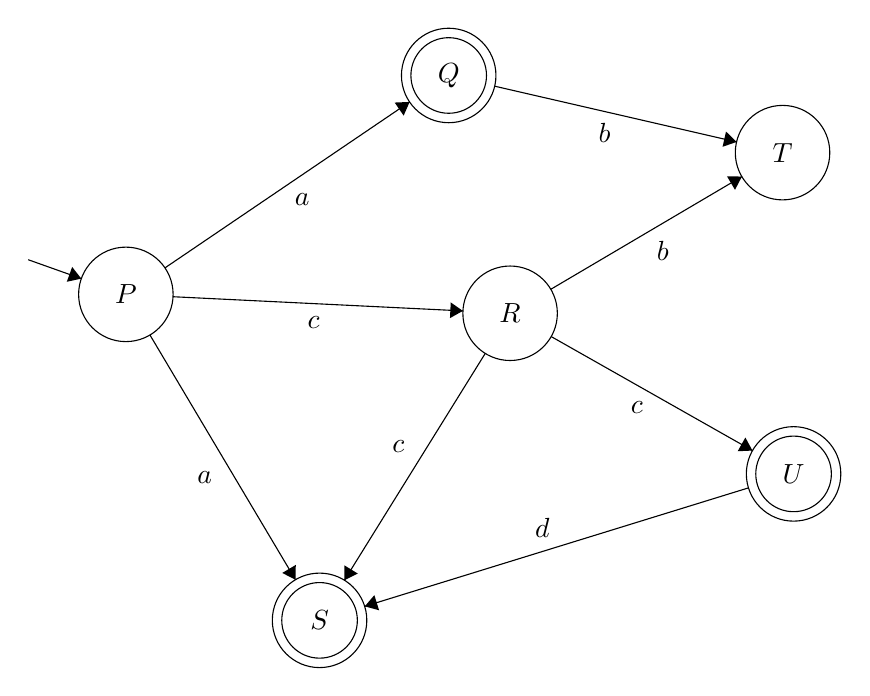
\begin{tikzpicture}[scale=0.2]
				\tikzstyle{every node}+=[inner sep=0pt]
				\draw [black] (9.4,-29.6) circle (3);
				\draw (9.4,-29.6) node {$P$};
				\draw [black] (29.9,-15.7) circle (3);
				\draw (29.9,-15.7) node {$Q$};
				\draw [black] (29.9,-15.7) circle (2.4);
				\draw [black] (33.8,-30.8) circle (3);
				\draw (33.8,-30.8) node {$R$};
				\draw [black] (21.7,-50.3) circle (3);
				\draw (21.7,-50.3) node {$S$};
				\draw [black] (21.7,-50.3) circle (2.4);
				\draw [black] (51.1,-20.6) circle (3);
				\draw (51.1,-20.6) node {$T$};
				\draw [black] (51.8,-41) circle (3);
				\draw (51.8,-41) node {$U$};
				\draw [black] (51.8,-41) circle (2.4);
				\draw [black] (3.2,-27.4) -- (6.57,-28.6);
				\fill [black] (6.57,-28.6) -- (5.99,-27.86) -- (5.65,-28.8);
				\draw [black] (11.88,-27.92) -- (27.42,-17.38);
				\fill [black] (27.42,-17.38) -- (26.47,-17.42) -- (27.04,-18.25);
				\draw (20.6,-23.15) node [below] {$a$};
				\draw [black] (10.93,-32.18) -- (20.17,-47.72);
				\fill [black] (20.17,-47.72) -- (20.19,-46.78) -- (19.33,-47.29);
				\draw (14.9,-41.21) node [left] {$a$};
				\draw [black] (12.4,-29.75) -- (30.8,-30.65);
				\fill [black] (30.8,-30.65) -- (30.03,-30.11) -- (29.98,-31.11);
				\draw (21.33,-30.95) node [below] {$c$};
				\draw [black] (32.82,-16.38) -- (48.18,-19.92);
				\fill [black] (48.18,-19.92) -- (47.51,-19.26) -- (47.29,-20.23);
				\draw (39.8,-18.73) node [below] {$b$};
				\draw [black] (36.38,-29.28) -- (48.52,-22.12);
				\fill [black] (48.52,-22.12) -- (47.57,-22.1) -- (48.08,-22.96);
				\draw (43.5,-26.2) node [below] {$b$};
				\draw [black] (36.41,-32.28) -- (49.19,-39.52);
				\fill [black] (49.19,-39.52) -- (48.74,-38.69) -- (48.25,-39.56);
				\draw (41.85,-36.4) node [below] {$c$};
				\draw [black] (48.93,-41.89) -- (24.57,-49.41);
				\fill [black] (24.57,-49.41) -- (25.48,-49.66) -- (25.18,-48.7);
				\draw (35.85,-45.1) node [above] {$d$};
				\draw [black] (32.22,-33.35) -- (23.28,-47.75);
				\fill [black] (23.28,-47.75) -- (24.13,-47.33) -- (23.28,-46.81);
				\draw (27.12,-39.26) node [left] {$c$};
				\end{tikzpicture}
			\end{center}
			\caption{An example of an NFA}
      \label{pic_ex_nfa}
			\end{figure}
%%%end of nfa picture

	\subsection{Deterministic Finite Automaton}
	\label{defDFA}
  A~\emph{deterministic finite automaton} (DFA) is a special case of an NFA, where $\delta$ is a partial function 
$\delta: Q\times \Sigma \to Q$ and $|I| \leq 1$. To be precise, we give the whole definition of DFA.\newline
\newline
		A DFA is a quintuple $\mathcal{A}=(Q,\Sigma,\delta,I,F)$ where
		\begin{itemize}
			\item $Q$ is a finite set of states,
			\item $\Sigma$ is  an alphabet,
			\item $\delta$:  $Q \times \Sigma \to Q$ is a partial transition function. We use $p \xrightarrow{a} q$ to denote that $\delta(p,a)=q$
			\item $I\subseteq Q$ is finite set of initial states, that $|I| \leq 1$.
			\item $F\subseteq Q$ is finite set of final states.
		\end{itemize}
    An example of a DFA is given on the figure \ref{pic_ex_dfa}.


%%%example of DFA
\begin{figure}[t]
\begin{center}
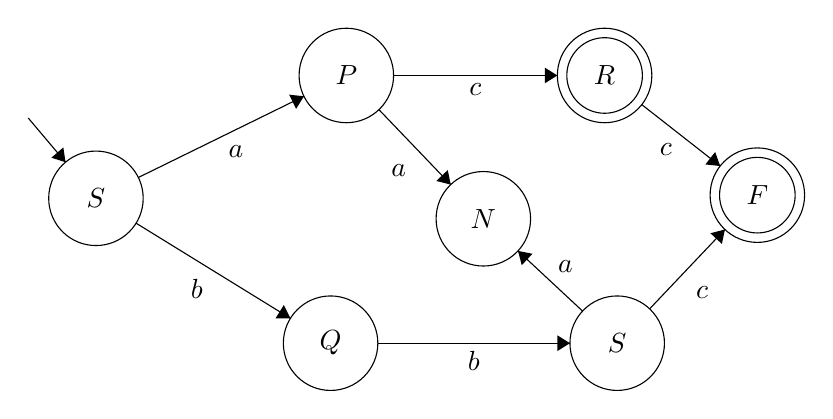
\begin{tikzpicture}[scale=0.2]
\tikzstyle{every node}+=[inner sep=0pt]
\draw [black] (9.9,-28) circle (3);
\draw (9.9,-28) node {$S$};
\draw [black] (25.8,-20.2) circle (3);
\draw (25.8,-20.2) node {$P$};
\draw [black] (24.8,-37.2) circle (3);
\draw (24.8,-37.2) node {$Q$};
\draw [black] (42.2,-20.2) circle (3);
\draw (42.2,-20.2) node {$R$};
\draw [black] (42.2,-20.2) circle (2.4);
\draw [black] (43,-37.2) circle (3);
\draw (43,-37.2) node {$S$};
\draw [black] (51.9,-27.8) circle (3);
\draw (51.9,-27.8) node {$F$};
\draw [black] (51.9,-27.8) circle (2.4);
\draw [black] (34.5,-29.3) circle (3);
\draw (34.5,-29.3) node {$N$};
\draw [black] (5.6,-22.9) -- (7.97,-25.71);
\fill [black] (7.97,-25.71) -- (7.83,-24.77) -- (7.07,-25.42);
\draw [black] (12.59,-26.68) -- (23.11,-21.52);
\fill [black] (23.11,-21.52) -- (22.17,-21.42) -- (22.61,-22.32);
\draw (18.79,-24.6) node [below] {$a$};
\draw [black] (12.45,-29.58) -- (22.25,-35.62);
\fill [black] (22.25,-35.62) -- (21.83,-34.78) -- (21.3,-35.63);
\draw (16.3,-33.1) node [below] {$b$};
\draw [black] (28.8,-20.2) -- (39.2,-20.2);
\fill [black] (39.2,-20.2) -- (38.4,-19.7) -- (38.4,-20.7);
\draw (34,-20.7) node [below] {$c$};
\draw [black] (27.8,-37.2) -- (40,-37.2);
\fill [black] (40,-37.2) -- (39.2,-36.7) -- (39.2,-37.7);
\draw (33.9,-37.7) node [below] {$b$};
\draw [black] (45.06,-35.02) -- (49.84,-29.98);
\fill [black] (49.84,-29.98) -- (48.92,-30.22) -- (49.65,-30.9);
\draw (47.98,-33.97) node [right] {$c$};
\draw [black] (44.56,-22.05) -- (49.54,-25.95);
\fill [black] (49.54,-25.95) -- (49.22,-25.06) -- (48.6,-25.85);
\draw (46.09,-24.5) node [below] {$c$};
\draw [black] (27.87,-22.37) -- (32.43,-27.13);
\fill [black] (32.43,-27.13) -- (32.24,-26.21) -- (31.51,-26.9);
\draw (29.62,-26.22) node [left] {$a$};
\draw [black] (40.8,-35.16) -- (36.7,-31.34);
\fill [black] (36.7,-31.34) -- (36.94,-32.25) -- (37.62,-31.52);
\draw (39.72,-32.76) node [above] {$a$};
\end{tikzpicture}
\end{center}
\caption{An example of an DFA}
\label{pic_ex_dfa}
\end{figure}
%%%%end of DFA example

  \subsection{$\epsilon$ transition}
  \label{defEpsTrans}
  $\epsilon$ transition of NFA $\mathcal{A}=(Q,\Sigma,\delta,I,F)$ is a transition $(p,\epsilon,q)\in\delta$ where $p,q\in Q$ and 
  $\epsilon$ is an empty word. $\epsilon$ transition is possible only in NFA.

%%%comment
\begin{comment}
	\subsection{Function $\hat{\delta}$}
	\label{defFunct}
		\begin{definition}
		A function $\hat{\delta}$ is define as
		\begin{description}
			$\hat{\delta}: Q\times\Sigma^{*}\rightarrow Q$
		\end{description}

		from $\delta$ by induction on the length of $x$:
			\begin{itemize}
				\item $\hat{\delta}(q,\epsilon)=q$, where $\epsilon$ is empty string
				\item $\hat{\delta}(q,xa)=\delta(\hat{\delta}(q,x),a)$
			\end{itemize}
		\end{definition}
\end{comment}
%%%%		


  \subsection{Operations over Finite Automata}
    \subsubsection{Automata Union}
    \label{defAUnion}
      Given a pair of NFA $\mathcal{A}=(Q_\mathcal{A},\Sigma,\delta_\mathcal{A},I_\mathcal{A},F_\mathcal{A})$ 
      and $\mathcal{B}=(Q_\mathcal{B},\Sigma,\delta_\mathcal{B},I_\mathcal{B},F_\mathcal{B})$. Their union is defined by
      \begin{description}
        \item $\mathcal{A} \cup \mathcal{B}=(Q_\mathcal{A}\cup Q_\mathcal{B},\Sigma,
            \delta_\mathcal{A}\cup\delta_\mathcal{B},I_\mathcal{A}\cup I_\mathcal{B},F_\mathcal{A}\cup F_\mathcal{B})$
      \end{description}
    
    \subsubsection{Automata Intersection}
    \label{defAInter}
      Given a pair of NFA, $\mathcal{A}=(Q_\mathcal{A},\Sigma,\delta_\mathcal{A},I_\mathcal{A},F_\mathcal{A})$ 
      and $\mathcal{B}=(Q_\mathcal{B},\Sigma,\delta_\mathcal{B},I_\mathcal{B},F_\mathcal{B})$. Their intersection is defined by
      \begin{description}
        \item $\mathcal{A} \cap \mathcal{B}=(Q_\mathcal{A}\cap Q_\mathcal{B},\Sigma,\delta,I_\mathcal{A}\cap I_\mathcal{B},F_\mathcal{A}\cap F_\mathcal{B})$\
      \end{description}
      where $\delta$ is defined by
      \begin{description}
        \item $\delta = 
        \{(p_1,q_1) \xrightarrow{a} (p_2,q_2)\ |\ p_1 \xrightarrow{a} p_2 \in \delta_\mathcal{A} \wedge q_1 \xrightarrow{a} q_2 \in \delta_\mathcal{B})\}$\
      \end{description}

      \subsubsection{Automata Product}
      \label{defAutProd}
      Given a pair of NFA, $\mathcal{A}=(Q_\mathcal{A},\Sigma,\delta_\mathcal{A},I_\mathcal{A},F_\mathcal{A})$ 
      and $\mathcal{B}=(Q_\mathcal{B},\Sigma,\delta_\mathcal{B},I_\mathcal{B},F_\mathcal{B})$. Their product is defined by
      \begin{description}
        \item $\mathcal{A} \times \mathcal{B}=
          (Q_\mathcal{A}\times Q_\mathcal{B},\Sigma,\delta,I_\mathcal{A}\times I_\mathcal{B},F_\mathcal{A}\times F_\mathcal{B})$\
      \end{description}
      where $\delta$ is defined by
      \begin{description}
        \item $\delta = 
        \{(p_1,q_1) \xrightarrow{a} (p_2,q_2)\ |\ p_1 \xrightarrow{a} p_2 \in \delta_\mathcal{A} \wedge q_1 \xrightarrow{a} q_2 \in \delta_\mathcal{B})\}$\
      \end{description}

  \subsubsection{Subset construction}
	\label{subset}
	Now we will define how to construct equivalent DFA $\mathcal{A}_{det}$ for a given NFA $\mathcal{A}=(Q,\Sigma,\delta,S,F)$. 
  \newline
  \newline
	\label{defSubset}
	$\mathcal{A}_{det}=(2^Q,\Sigma,\delta_{det},S,F_{det})$, where
	\begin{itemize}
		\item $2^Q$ is power set of $Q$
		\item $F_{det}=\{Q'\subseteq Q\ |\ Q'\cap F \not = \varnothing\}$
		\item $\delta_{det}(Q',a)=\bigcup\limits_{q\in Q'}\delta(q,a)$, where $a\in\Sigma$
	\end{itemize}

  This classical (so-called \emph{textbook}) approach is called \emph{subset construction}.
    An example of this approach is shown on the figure \ref{pic_sub}.
	
	%%%%example of NFA to DFA	
	\begin{figure}[t]
\begin{center}
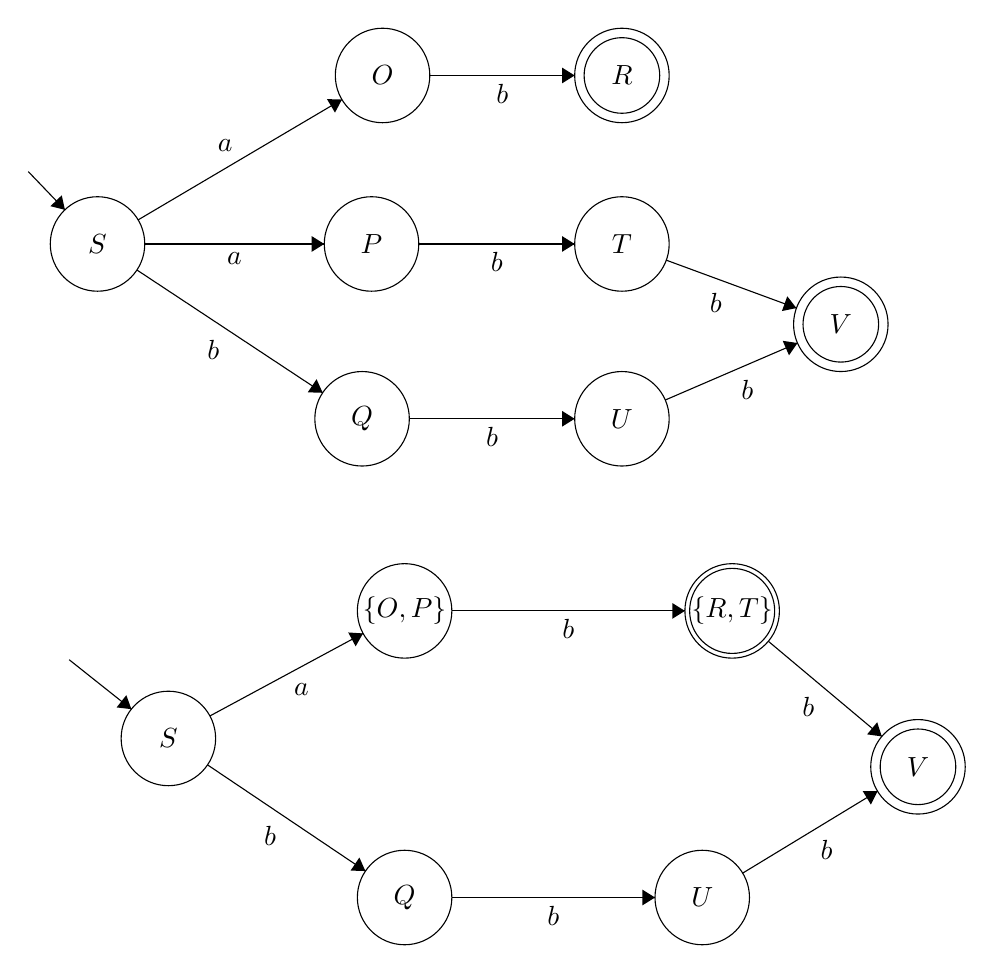
\begin{tikzpicture}[scale=0.2]
\tikzstyle{every node}+=[inner sep=0pt]
\draw [black] (7.9,-14.8) circle (3);
\draw (7.9,-14.8) node {$S$};
\draw [black] (26,-4.1) circle (3);
\draw (26,-4.1) node {$O$};
\draw [black] (25.3,-14.8) circle (3);
\draw (25.3,-14.8) node {$P$};
\draw [black] (24.7,-25.9) circle (3);
\draw (24.7,-25.9) node {$Q$};
\draw [black] (41.2,-4.1) circle (3);
\draw (41.2,-4.1) node {$R$};
\draw [black] (41.2,-4.1) circle (2.4);
\draw [black] (41.2,-14.8) circle (3);
\draw (41.2,-14.8) node {$T$};
\draw [black] (41.2,-25.9) circle (3);
\draw (41.2,-25.9) node {$U$};
\draw [black] (55.1,-19.9) circle (3);
\draw (55.1,-19.9) node {$V$};
\draw [black] (55.1,-19.9) circle (2.4);
\draw [black] (12.4,-46.2) circle (3);
\draw (12.4,-46.2) node {$S$};
\draw [black] (27.4,-38.1) circle (3);
\draw (27.4,-38.1) node {$\{O,P\}$};
\draw [black] (27.4,-56.3) circle (3);
\draw (27.4,-56.3) node {$Q$};
\draw [black] (48.2,-38.1) circle (3);
\draw (48.2,-38.1) node {$\{R,T\}$};
\draw [black] (48.2,-38.1) circle (2.7);
\draw [black] (46.3,-56.3) circle (3);
\draw (46.3,-56.3) node {$U$};
\draw [black] (60,-48) circle (3);
\draw (60,-48) node {$V$};
\draw [black] (60,-48) circle (2.4);
\draw [black] (3.5,-10.2) -- (5.83,-12.63);
\fill [black] (5.83,-12.63) -- (5.63,-11.71) -- (4.91,-12.4);
\draw [black] (10.48,-13.27) -- (23.42,-5.63);
\fill [black] (23.42,-5.63) -- (22.47,-5.6) -- (22.98,-6.46);
\draw (16,-8.95) node [above] {$a$};
\draw [black] (10.9,-14.8) -- (22.3,-14.8);
\fill [black] (22.3,-14.8) -- (21.5,-14.3) -- (21.5,-15.3);
\draw (16.6,-15.3) node [below] {$a$};
\draw [black] (10.4,-16.45) -- (22.2,-24.25);
\fill [black] (22.2,-24.25) -- (21.81,-23.39) -- (21.25,-24.22);
\draw (15.25,-20.85) node [below] {$b$};
\draw [black] (29,-4.1) -- (38.2,-4.1);
\fill [black] (38.2,-4.1) -- (37.4,-3.6) -- (37.4,-4.6);
\draw (33.6,-4.6) node [below] {$b$};
\draw [black] (28.3,-14.8) -- (38.2,-14.8);
\fill [black] (38.2,-14.8) -- (37.4,-14.3) -- (37.4,-15.3);
\draw (33.25,-15.3) node [below] {$b$};
\draw [black] (27.7,-25.9) -- (38.2,-25.9);
\fill [black] (38.2,-25.9) -- (37.4,-25.4) -- (37.4,-26.4);
\draw (32.95,-26.4) node [below] {$b$};
\draw [black] (43.95,-24.71) -- (52.35,-21.09);
\fill [black] (52.35,-21.09) -- (51.41,-20.95) -- (51.81,-21.87);
\draw (49.17,-23.41) node [below] {$b$};
\draw [black] (44.02,-15.83) -- (52.28,-18.87);
\fill [black] (52.28,-18.87) -- (51.7,-18.12) -- (51.36,-19.06);
\draw (47.17,-17.88) node [below] {$b$};
\draw [black] (6.1,-41.2) -- (10.05,-44.34);
\fill [black] (10.05,-44.34) -- (9.73,-43.45) -- (9.11,-44.23);
\draw [black] (15.04,-44.77) -- (24.76,-39.53);
\fill [black] (24.76,-39.53) -- (23.82,-39.47) -- (24.29,-40.35);
\draw (20.85,-42.65) node [below] {$a$};
\draw [black] (14.89,-47.88) -- (24.91,-54.62);
\fill [black] (24.91,-54.62) -- (24.53,-53.76) -- (23.97,-54.59);
\draw (18.85,-51.75) node [below] {$b$};
\draw [black] (30.4,-38.1) -- (45.2,-38.1);
\fill [black] (45.2,-38.1) -- (44.4,-37.6) -- (44.4,-38.6);
\draw (37.8,-38.6) node [below] {$b$};
\draw [black] (30.4,-56.3) -- (43.3,-56.3);
\fill [black] (43.3,-56.3) -- (42.5,-55.8) -- (42.5,-56.8);
\draw (36.85,-56.8) node [below] {$b$};
\draw [black] (48.87,-54.75) -- (57.43,-49.55);
\fill [black] (57.43,-49.55) -- (56.49,-49.54) -- (57.01,-50.4);
\draw (54.2,-52.65) node [below] {$b$};
\draw [black] (50.5,-40.03) -- (57.7,-46.07);
\fill [black] (57.7,-46.07) -- (57.41,-45.17) -- (56.77,-45.94);
\draw (53.04,-43.54) node [below] {$b$};
\end{tikzpicture}
\end{center}
	\caption{A simple example of NFA to DFA conversion via the subset construction. 
    Here is shown small NFA with small $\Sigma$, but for larger NFA could state explosion occur.}
    \label{pic_sub}
	\end{figure}
	%%%end of NFA to DFA



	\subsection{Run of Finite Automaton}
	\label{defRun}
  A~\emph{run} of an NFA $\mathcal{A}=(Q,\Sigma,\delta,I,F)$ from a state $q$
  over a word $w=a_1\ldots a_n$ is a sequence $r = q_0 \ldots q_n$, where $\forall\,0\leq i \leq n\ .\ q_i\in Q$ 
  such that $q_0=q$ and $(q_i,a_{i+1},q_{i+1})\in \delta$. 
  The run $r$ is called \emph{accepting} iff $q_n \in F$. 
	An word $w \in \Sigma^{*}$ is called \emph{accepting}, if there exists an \emph{accepting} run for $w$.
  An \emph{unreachable} state $q$ of an NFA $\mathcal{A}=(Q,\Sigma,\delta,I,F)$ is a state for which there is no run $r=q_0\ldots q$ of 
  $\mathcal{A}$ over a word $w \in \Sigma^{*}$ 
  such that $q_0\in I$.
  An \emph{useless} (also called nonterminating) state $q$ of an NFA $\emph{A}=(Q,\Sigma,\delta,I,F)$ is state that there is no run $r=q\ldots q_n$ 
  of $\emph{A}$ over a word
  $w \in \Sigma^{*}$ such that $q_n \in F$.
  Given a pair of states $p,q$ of an NFA $\emph{A}=(Q,\Sigma,\delta,I,F)$, these states are equivalent if 
  $\forall w \in \Sigma^{*}: \emph{ Run from } p \emph{ over } w \emph{ is accepting} \Leftrightarrow 
			\emph{ Run from } q \emph{ over } w \emph{ is accepting}$.


  \subsection{Complete DFA}
  \label{defCompleteDFA}
  \emph{Complete} DFA $\mathcal{A_C}=(Q_C,\Sigma,\delta_C,I_C,F_C)$ is DFA where $\forall p\in Q_C\,\forall a\in \Sigma\ \exists\, q\in Q_C :
  p\xrightarrow{a}q\in\delta_C$. 
  It is possible to create complete DFA $\mathcal{A_C}=(Q_C,\Sigma,\delta_C,I_C,F_C)$ from DFA $\mathcal{A}=(Q,\Sigma,\delta,I,F)$ such that $Q_C=Q\cup\{q\}$, 
  $I_C=I$, $F_C=F$, 
  $\delta_C = \delta \cup \{p\xrightarrow{a}q\,|\,a\in\Sigma,p\in Q_C,p\xrightarrow{a}r\not\in\delta,r\in Q\}$.

	\subsection{Minimal DFA}
	\label{defMinDFA}
		Minimal DFA $\mathcal{A}=(Q,\Sigma,\delta,I,F)$ is complete DFA which satisfies this conditions:
		\begin{itemize}
			\item There are no unreachable states
			\item There is maximal one nonterminating state
			\item Equivalent states are collapsed
		\end{itemize}


  \subsection{Language of Finite Automaton}
  Let have a NFA $\mathcal{A}=(Q,\Sigma,\delta,I,F)$.
  The~\emph{language} of a state $q \in Q$ is defined as 
  $L_\mathcal{A}(q) = \{w\in \Sigma^{*}\ |\ $\emph{there exists an accepting run of }$
  \mathcal{A}$$ 
  \emph{ from }q\emph{ over }w\}$, while the language of a set of states $R\subseteq Q$ is defined as $L_{\mathcal{A}}(R)=\bigcup_{q\in R}L_{\mathcal{A}}(q)$.
  The language of an NFA $\mathcal{A}$ is defined as $L_{\mathcal{A}}=L_{\mathcal{A}}(I)$.

\section{Regular Languages}
		A language $L$ is \emph{regular}, if there exists an NFA $\mathcal{A}=(Q,\Sigma,\delta,I,F)$, such that $L=L_\mathcal{A}$.

    \subsection{Closure Properties}
    Regular languages are closed under certain operation if result of this operation over some regular language is always regular language too.

		Let introduce the closure properties of regular languages on an alphabet $\Sigma$:
		\begin{itemize}
			\item Union:  $L_1 \cup L_2$\\%=\{x\ |\ x \in L_1 \vee x\in L_2\}$
      Union of two NFA is described in section \ref{defAUnion}.
			\item Intersection:  $L_1 \cap L_2$\\%=\{x\ |\ x \in L_1 \wedge x\in L_2\}$
      Intersection of two NFA is described in section \ref{defAInter}.
			\item Complement: $\overline{L}$\\%=\{x\ |\ x\not\in L\}$
      Complement of NFA $\mathcal{A}$ is done by its determinizing (via subset construction described in section \ref{subset}), completion of this DFA (via
      method described in \ref{defCompleteDFA}) and switching its final and non-final states set.

      \item Difference: $L_1-L_2$\\%=\{x\ |\ x\in L \wedge x\not\in K\}$
      Difference of NFA $\mathcal{A}=(Q_\mathcal{A},\Sigma,\delta_\mathcal{A},I_\mathcal{A},F_\mathcal{A})$ 
      and NFA $\mathcal{B}=(Q_\mathcal{B},\Sigma,\delta_\mathcal{B},I_\mathcal{B},F_\mathcal{B})$ is done by creating
      complete DFA $\mathcal{A_C}$ and $\mathcal{B_C}$ (by methods \ref{subset} and \ref{defCompleteDFA}) 
      and creating product DFA (created as is described in section 
      \ref{defAutProd})
      $\mathcal{A_C} \times \mathcal{B_C}=
          (Q_{\mathcal{A}_C}\times Q_{\mathcal{B}_C},\Sigma,\delta_{{\mathcal{A}_C}\times{\mathcal{B}_C}},I_{\mathcal{A}_C}\times I_{\mathcal{B}_C},F)$
      where $F=\{(p,q)\,|\, p\in F_{\mathcal{A}_C} \wedge q\not\in F_{\mathcal{B}_C}\}$.

			\item Reversal: $\{a_1\dots a_n \in L \ |\ y=a_n\dots a_1 \in L\}$\\
      Reversion of a NFA $\mathcal{A}=(Q_\mathcal{A},\Sigma,\delta_\mathcal{A},I_\mathcal{A},F_\mathcal{A})$ is
      NFA $\mathcal{A}_{rev}=(Q_{\mathcal{A}_{rev}},\Sigma,\delta_{\mathcal{A}_{rev}},I_{\mathcal{A}_{rev}},F_{\mathcal{A}_{rev}})$ 
      where $Q_{\mathcal{A}_{rev}} = Q_\mathcal{A}$, 
      $I_{\mathcal{A}_{rev}} = F_\mathcal{A}$, $F_{\mathcal{A}_{rev}} = I_\mathcal{A}$ and 
      $\delta_{\mathcal{A}_{rev}}=\{(q,a,p)\,|\,p,q \in Q_\mathcal{A}, a \in \Sigma,(p,a,q)\in\delta_{\mathcal{A}}\}$ .

      \item Iteration: $L^{*}$\\ %: $L^{*}$
      Iteration of a NFA $\mathcal{A}=(Q_\mathcal{A},\Sigma,\delta_\mathcal{A},I_\mathcal{A},F_\mathcal{A})$ 
      is NFA $\mathcal{A}^{*}=(Q_\mathcal{A},\Sigma,\delta_\mathcal{A}^{*},I_\mathcal{A},F_\mathcal{A})$ where $\delta_\mathcal{A}^{*}=\delta_\mathcal{A}\cup
      \{(i_\mathcal{A},\epsilon,f_\mathcal{A})\,|\,i_\mathcal{A}\in I_\mathcal{A},f_\mathcal{A}\in F_\mathcal{A}\} \cup 
      F_\mathcal{A}\times \{\epsilon\} \times I_\mathcal{A}$

			\item Concatenation: $L\cdot K=\{x \cdot y\ |\ x\in L \wedge y\in K\}$\\
      Concatenation of a NFA $\mathcal{A}=(Q_\mathcal{A},\Sigma,\delta_\mathcal{A},I_\mathcal{A},F_\mathcal{A})$ and a NFA 
      $\mathcal{B}=(Q_\mathcal{B},\Sigma,\delta_\mathcal{B},I_\mathcal{B},F_\mathcal{B})$ is 
      NFA $\mathcal{A}\cdot\mathcal{B}=(Q_\mathcal{A}\cup Q_\mathcal{B},\Sigma,\delta,I_\mathcal{A},F_\mathcal{B})$ where $\delta=\delta_\mathcal{A} \cup
      \delta_\mathcal{B} \cup F_\mathcal{A}\times\{\epsilon\}\times I_\mathcal{B}$.

  \end{itemize}

\begin{comment}
		\subsection{Union, intersection, inclusion}
\label{defOP}
		\begin{definition}
		Let $L_1$ and $L_2$ be languages. \emph{Union, intersection, inclusion} are defined as:
		\begin{description*}
			\item [$Union:$]  $L_1 \cup L_2=\{x\ |\ x \in L_1 \vee x\in L_2\}$
			\item [$Intersection:$]  $L_1 \cap L_2=\{x\ |\ x \in L_1 \wedge x\in L_2\}$
			\item [$Inclusion:$]  $L_1 \subseteq L_2 \Leftrightarrow L_1 \cap \overline{L_2}=\varnothing$
		\end{description*}
		\end{definition}
		
\end{comment}

\chapter{Inclusion Checking over NFA}
\label{chapInclusion}
Given a pair of NFA $\mathcal{A}=(Q_\mathcal{A},\Sigma,\delta_\mathcal{A},I_\mathcal{A},F_\mathcal{A})$ 
and $\mathcal{B}=(Q_\mathcal{B},\Sigma,\delta_\mathcal{B},I_\mathcal{B},F_\mathcal{B})$, 
the \emph{language inclusion problem} is decision whether $L_\mathcal{A} \subseteq L_\mathcal{B}$ what is defined by standard set operations as
$L_\mathcal{A}\cap \overline{L_\mathcal{B}} = \varnothing$.
This problem is PSPACE-complete \cite{cav06}. The \emph{textbook} algorithm for checking inclusion $L_\mathcal{A}\subseteq L_\mathcal{B}$ works by first 
determinizing $\mathcal{B}$ (yielding the DFA 
$\mathcal{B}_{det}$ using subset construction algorithm \ref{subset}), 
complementing it ($\overline{\mathcal{B}_{det}}$) and constructing the NFA $\mathcal{A} \times \overline{\mathcal{B}_{det}}$ 
accepting the intersection of $L_{\mathcal{A}}$ and ${L_{\overline{\mathcal{B}_{det}}}}$ and
checking whether its language is nonempty. Any accepting run in this automaton may serve as a witness that the inclusion between $\mathcal{A}$ 
and $\mathcal{B}$ does not hold.
Some recently introduced approaches (so-called antichains \cite{cav06}, its optimization using simulation \cite{tacas10} and so-called bisimulation up to
congruence \cite{popl13}) avoid the explicit construction of $\overline{\mathcal{B}_{det}}$ and the related state explosion in many cases.

We have to define following terms for the further description of the new techniques for the inclusion checking.
We denote product state of an NFA $\mathcal{A} \times \mathcal{B}$ as a pair $(p,P)$ of a state $p\in Q_\mathcal{A}$ and a macrostate $P \subseteq Q_\mathcal{B}$.
We define post-image of the product state $(p,P)$ of a NFA $\mathcal{A}\times \mathcal{B}$ by:\
$Post((p,P)):=\{(p',P')\ |\ \exists a \in \Sigma: (p,a,p')\in \delta_\mathcal{A}, P'=\{p''\ |\ \exists p \in P:(p,a,p'')\in \delta_\mathcal{B}\}\}$

\section{Checking Inclusion with Antichains and Simulation}
\label{sectionAntichain}
We define an antichain, simulation and some others terms before describing the algorithm itself.

Given a partially ordered set $Y$, an \emph {antichain} is a set $X \subseteq Y$ such that all elements of $X$ are incomparable.

A~forward \emph{simulation} on the NFA $\mathcal{A}$ is a relation $\preceq\  \subseteq Q_1 \times Q_1$ 
such that if $p \preceq r$ then (i) $p \in F_1 
\Rightarrow r \in F_1$ and (ii) for every transition $p\xrightarrow{a}p'$, there exists a transition 
$r\xrightarrow{a}r'$ such that $p' \preceq r'$. Note that simulation implies language inclusion, i.e., $p\preceq q \Rightarrow L_\mathcal{A}(p)
\subseteq L_\mathcal{A}(q)$ \cite{focs95}. %TODO citovate?


%Let denote $A^{\subseteq}$ as the set of relations over automaton $A$ that imply inclusion,\\ so if $\preceq \in A^{\subseteq}$, 
%then $p\preceq r \Rightarrow L(A)(p) \subseteq L(A)(r)$.
%
For two macro-states $P$ and $R$ of a NFA is $R\preceq^{\forall\exists}P$ shorthand for $\forall r\in R.\exists p \in P: r \preceq p$.

Product state $(p,P)$ is accepting, if $p$ is accepting in automaton $A$ and $P$ is rejecting in automaton $B$.

\subsection{Antichain Algorithm Description}
The antichains algorithm \cite{cav06} starts searching for a final state of the automaton $\mathcal{A}\times \overline{\mathcal{B}_{det}}$ while
pruning out the states which are not necessary to explore. $\mathcal{A}$ is explored nondeterministically and $\mathcal{B}$ 
is gradually determinized, so the algorithm explores pairs $(p,P)$ where $p\in Q_\mathcal{A}$ and $P \subseteq Q_\mathcal{B}$. 
The antichains algorithm derives new states along the product automaton transitions and inserts them to the set of visited pairs $X$.
$X$ keeps only minimal elements with respect to the ordering given by $(r,R)\sqsubseteq (p,P)$ iff $r=p \wedge R \subseteq P$. 
If there is generated a pair $(p,P)$ and there is 
$(r,R)\in X$ such that $(r,R) \sqsubseteq (p,P)$, we can skip $(p,P)$ and not insert it to $X$ for further search.
 
An improvement of the antichains algorithm using simulation \cite{tacas10} is based on the following optimization. 
We can stop the search from a pair $(p,P)$ if either (a) there exists some already visited pair $(r,R) \in X$ 
such that $p\preceq r \wedge R\preceq^{\forall\exists}P$, 
or (b) there is $p' \in P$ such that $p \preceq p'$. This first
optimization is in algorithm \ref{algAntichain} at lines 11--14.

Another optimization \cite{tacas10} of the antichain algorithm is based on the fact 
that $L_\mathcal{A}(P)=L_\mathcal{A}(P-\{p_1\})$ if there exists $p_2 \in P$, such as $p_1 \preceq p_2$. We can remove the state $p_1$ 
from macrostate $P$, because if $L_\mathcal{A}(P)$ rejects the word 
then $L_\mathcal{A}(P-\{p_1\})$ rejects this word too. This optimization is applied by the function $Minimize$ at
the lines 4 and 7 in the algorithm \ref{algAntichain}.

The whole pseudocode of the antichain algorithm is given as algorithm \ref{algAntichain}.

\begin{algorithm}[H]
	\label{algAntichain}
	\KwIn{NFA's $\mathcal{A}=(Q_A,\Sigma,\delta_A,I_A,F_A),\ \mathcal{B}=(Q_B,\Sigma,\delta_B,I_B,F_B)$.\\ 
	 A relation $\preceq \in (\mathcal{A} \cup \mathcal{B})^{\subseteq}$.}
	\KwOut{TRUE if $\mathcal{L(A)}\subseteq\mathcal{L(B)}$. Otherwise, FALSE.}
		\If{there is an accepting product-state in \{$(i,I_{\mathcal{B}})|i\in I_{\mathcal{A}}$\}}
			{return FALSE\;}
		$Processed$:=$\varnothing$\;
		$Next$:= Initialize(\{$(s,Minimize(I_B))\mid s\in I_A$\})\;
		\While{($Next\neq \varnothing$)}
		{
			Pick and remove a product-state $(r,R)$ from Next and move it to Processed\;
			\ForAll{$(p,P)\in \{(r',Minimize(R'))\mid (r',R')\in Post((r,R))\}$}
			{
				\eIf{$(p,P)$ is an accepting product-state}
				{
					\Return FALSE\;}
					{
						\If{$\not{\exists}p'\in P\ s.t.\ p\preceq p'$}
						{
							\If{$\not{\exists} (x,X) \in Processed\cup Next\ s.t.\ p\preceq x \wedge X\preceq^{\forall \exists}P$}
							{
							 Remove all $(x,X)$ from $Processed\cup Next\ s.t.\ x\preceq p \wedge P\preceq^{\forall \exists}X$\;
							 Add $(p,P)$ to $Next$\;
							}
						}
				 }
		  }
		}
		\Return TRUE;
	\caption{Language inclusion checking with antichains and simulations}
\end{algorithm}\
\begin{comment}
Let describe two optimization use in algorithm \ref{algAntichain} based on \cite{tacas10}. First optimization comes from the observation that
we can stop search from product-state $(p,P)$, if there exists some visited product state $(r,R)$, 
such that $p\preceq r \wedge R\preceq^{\forall\exists}P$, or $\exists p'\in P: p \preceq p'$. First part of condition says that 
if $(p,P)$ takes automaton to the accepting state, $(r,R)$ will be taken to accepting state too, so we do not have search from $(p,P)$. Second part of condition
shows, that every accepting word of $p$ takes $P$ to accepting state too, because $\exists p'\in P: p \preceq p'$.
Proof for this can be found in \cite{tacas10}. This first
optimization is in algorithm \ref{algAntichain} at lines 11--14.

Second optimization is based on fact, that $L(A)(P)=L(A)(P-\{p_1\})$, if there exists $p_2$, such as $p_1 \preceq p_2$. We can remove the state $p_1$ 
from macro-state $P$, because if $L(A)(P)$ rejects the word, then $L(A)(P-\{p_1\})$ rejects this word too. This optimization is applied in function $Minimize$ at
lines 4 and 7 in algorithm \ref{algAntichain}. Proof for this optimization is again in \cite{tacas10}.
\end{comment}

\section{Checking Inclusion with Bisimulation up to Congruence}
\label{sectionCongr}
Another approach to checking language inclusion of NFA is based on bisimulation up to congruence \cite{popl13}. The definition of congruence relation is
following:

	Let $X$ be a set with a n-ary operation $O$ over $X$. Congruence is an equivalence relation $R$, 
	which follows this condition $\forall a_1,\ldots,a_n,b_1,\ldots,b_n\in X$:
		\begin{description}
			\item $a_1 \sim_{R} b_1,\ldots,a_n \sim_{R} b_n \Rightarrow O_n(a_1,\ldots,a_n) \sim_{R} O_n(b_1,\ldots,b_n)$, where $a_i \in X, b_i \in X$
		\end{description}

This technique was originally developed for checking equivalence of languages of automata but it can
also be used for checking language inclusion, based on the observation that $L_\mathcal{A}\cup L_\mathcal{B}= L_\mathcal{B} 
\Leftrightarrow L_\mathcal{A}\subseteq L_\mathcal{B}$.

  This approach is based on the computation of a~\emph{congruence closure} $c(R)$ 
  for some binary relation on states of the determinized automaton $R \subseteq 2^Q\times 2^Q$ defined 
  %associative, commutative, idempotent binary operation $+: Q\times Q \to Q$ 
  as a relation $c(R)=(r\cup s\cup t \cup u\cup id)^{\omega}(R)$, where
  \begin{description}
  \item $id(R)=R$, 
  \item $r(R)=\{(X,X)\ |\ X\subseteq Q\}$, 
  \item $s(R)=\{(Y,X)\ |\ XRY\}$,
  \item $t(R)=\{(X,Z)\ |\ \exists\,Y\subseteq Q,\ XRYRZ\}$,
  \item $u(R)=\{(X_1 \cup X_2,Y_1\cup Y_2)\ |\ X_1 R Y_1 \wedge X_2 R Y_2\}$. 
  \end{description}



 \subsection{Congruence Algorithm Description}
\label{subsectCongr}
The congruence algorithm works on a similar principle as the antichains algorithm but 
it starts building not only $\mathcal{B}_{det}$ but also $\mathcal{A}_{det}$ because the original purpose of this algorithm is checking of 
language equivalence. States of a product automaton $\mathcal{A}_{det} \times \mathcal{B}_{det}$  (so-called product states) are the pairs 
$(P_\mathcal{A},P_\mathcal{B})$ of macrostate $P_\mathcal{A} \subseteq Q_\mathcal{A}$ and macrostate
$P_\mathcal{B} \subseteq Q_\mathcal{B}$. 
The algorithm searches for a victim that proves $L_\mathcal{A} \neq L_\mathcal{B}$. The victim is a product state $(P_\mathcal{A},P_\mathcal{B})$ 
which breaks a condition that
the $P_\mathcal{A}$ contains a final state of $A$ if and only if $P_\mathcal{B}$ contains a final state of $B$. 

The optimization brought by this algorithm is based on computing of a congruence closure of the set of already visited pairs of macrostates. 
If the generated pair is in the congruence closure, it can be skipped and further not processed.
	The whole pseudocode of the congruence algorithm is given as algorithm \ref{algCongr}.

	\begin{algorithm}[h]
		\label{algCongr}
		\KwIn{NFA's $A=(Q_A,\Sigma,\delta_A,I_A,F_A),\ B=(Q_B,\Sigma,\delta_B,I_B,F_B)$.} 
		\KwOut{TRUE, if $L(A)$ and $L(B)$ are in equivalence relation. Otherwise, FALSE.}
			$Processed$ := $\varnothing$\;
			$Next$ := $(I_A,I_B)$\;
			\While{$Next \neq \varnothing$}
			{
				Pick and remove a product state $(X,Y)$ from $Next$\;
				\If {($X$,$Y) \in c(Processed \cup Next)$}
				{skip\;}
				\If {$\neg(\{x\in X| x\in F_\mathcal{A}\} \neq \varnothing \Leftrightarrow \{y\in Y| y\in F_\mathcal{B}\}\neq \varnothing)$}
				{
					\Return FALSE\;
				}
				%\ForAll {$a\in \Sigma$}
				%{
					Add ($post(X,Y)$) to $Next$\;
				%}
				Add($X$,$Y$) to $Processed$\;
			}
			\Return TRUE;
		\caption{Language equivalence checking with congruence}
\end{algorithm}

Comparing the mentioned approaches to the checking language inclusion can be seen in Figure \ref{automata}.
\begin{figure}[bt]
\begin{center}
	\scalebox{1}
	{
		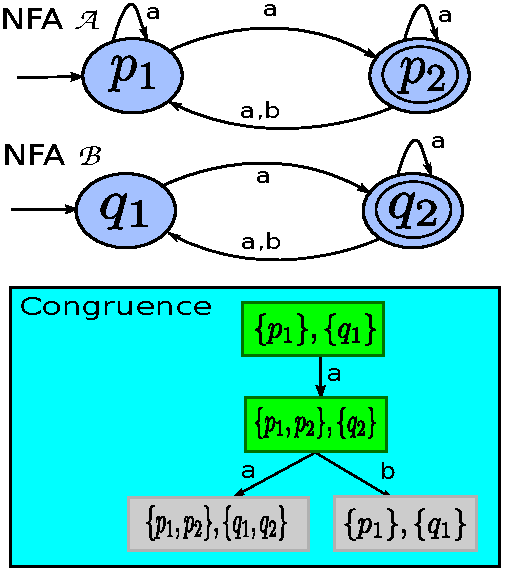
\includegraphics[scale=0.5]{fig/congr1.pdf}
		\hspace{0.55cm}
  	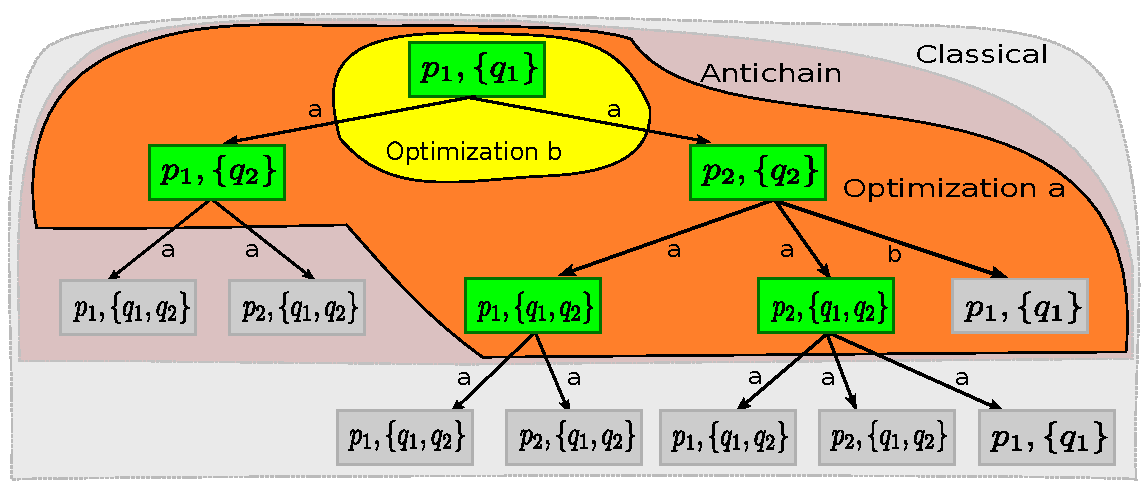
\includegraphics[scale=0.5]{fig/ac1.pdf}
	}
  \caption{
      \rm{
      \hspace{0.1cm} The figure is based on an example from \cite{tacas10}.
      It shows the procedure of checking language inclusion between two NFA using the mentioned approaches (which correspond to the labeled areas).
      %The labeled areas correspond to mentioned approaches.
      The antichain algorithm reduces number of the generated states compared with the classical,
      e.g., $(p_2,\{q_1,q_2\})$ is not further explored because $(p_2,\{q_2\}) \sqsubseteq (p_2,\{q_1,q_2\})$. 
      The optimization a and b are improvements of the antichain algorithm using simulation. 
      The congruence algorithm also reduces number of the generated states, so $(\{p_1,p_2\},\{q_1,q_2\})$ 
      is not further explored because it is in congruence closure 
      of the set of visited states.}}
      %It shows macrostates 
			%that are generated when checking language inclusion between two NFA using different approaches. Optimization a and b
			%correspond to the parts of the improvement of antichain algorithm using simulation.}}
  \label{automata}
\end{center}
\end{figure}

\subsection{Computation of Congruence Closure}
\label{subsectionCongr}
The computation of the congruence closure is crucial for performance and efficiency of the whole method. This thesis implements
an algorithm described by \cite{popl13} which is based on using of the so-called rewriting rules. For each pair of macrostates $(X,Y)$ in 
a relation $R$ of the visited macrostates exists two rewriting rules which has following form:
\begin{center}
$X\rightarrow X\cup Y$ \hspace{5cm} $Y\rightarrow X\cup Y$
\end{center}

These rules can be used for computation of a \emph{normal form} of a set of states \cite{popl13}. The normal form of a macrostate $X$ created with
the usage of rewriting rules of the relation $R$ is denoted as $X{\downarrow_R}$.
Checking if $(X,Y)\in c(R)$ using derivation of the normal form is based on the observation that $X{\downarrow_R}=Y{\downarrow_R}$ 
iff $(X,Y)\in c(R)$ \cite{popl13}.

An example (taken from \cite{popl13}) is given to illustrate an application of this approach for checking equivalency of 
NFA $\mathcal{A}=(Q_\mathcal{A},\Sigma,\delta_\mathcal{A},I_\mathcal{A},F_\mathcal{A})$ 
and $\mathcal{B}=(Q_\mathcal{B},\Sigma,\delta_\mathcal{B},I_\mathcal{B},F_\mathcal{B})$ (both NFA are on figure \ref{figHKCex}). 
Let have a relation $R=\{(\{x\},\{u\}),(\{y,z\},\{u\})\}$ of the visited product states and a newly generated product state 
$(\{x,y\},\{u\})$ (where $\{x,y\}\subseteq Q_\mathcal{A}$ and 
$\{u\} \subseteq Q_\mathcal{B}$). For checking of $(\{x,y\},\{u\})\in c(R)$ it is needed to compute the normal forms of the macrostates $\{x,y\}$ and $\{u\}$ 
A derivation of both normal forms is shown on \ref{figHKCRew}. 
The normal form of the set $\{x,y\}$ is derived in two steps.
At the first step is applied rule $\{x\}\rightarrow\{x,u\}$ (base on $(\{x\},\{u\})\in R$) so we get a set $\{x,y,u\}$. As the second one, rule 
$\{u\}\rightarrow\{y,z,u\}$ (based on product state $(\{y,z\},\{u\})\in R$) is applied, so the result is $\{x,y,z,u\}$. The normal form of the set $\{u\}$
is derived in two steps too. At the first step, a rule $\{u\}\rightarrow\{x,u\}$ is applied so we get a set $\{x,u\}$ and then rule 
$\{u\}\rightarrow\{y,z,u\}$  is used and the result set is $\{x,y,z,u\}$. The derived normal sets are equal so it holds that $(\{x,y\},u)\in c(R)$ and
it is not necessary to further explore product automaton $\mathcal{A}\times \mathcal{B}$ from this state.

\begin{figure}[bt]
\begin{center}
  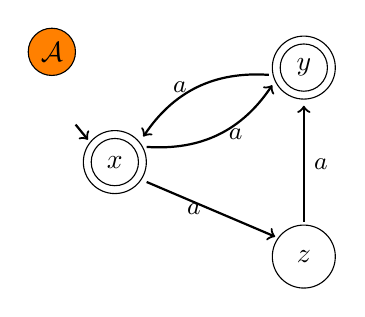
\begin{tikzpicture}
[
  scale=0.4
]

\draw (2,8.5)[fill=orange] circle (0.75);
\draw (2,8.5) node {$\mathcal{A}$};

\draw (4,5) circle (1);
\draw (4,5) circle (0.75);
\draw (4,5) node {$x$};
\draw (10,8) circle (1);
\draw (10,8) circle (0.75);
\draw (10,8) node {$y$};
\draw (10,2) circle (1);
\draw (10,2) node {$z$};

\node (s) at (2.5,6.5) {};
\node (sx) at (3.4,5.4) {};

\node (x) at (4.7,5.5) {};
\node (y) at (9.2,7.75) {};

\node (xz) at (4.7,4.5) {};
\node (z) at (9.4,2.5) {};

\node (yz) at (10,7.1) {};
\node (zy) at (10,2.8) {};

\path[->,thick,every node/.style={font=\sffamily\small}]
(x) edge [bend right] node[right] {$a$} (y)
(y) edge [bend right] node[left] {$a$} (x)

(xz) edge node[left] {$a$} (z)

(zy) edge node[right] {$a$} (yz)

(s) edge (sx);

\end{tikzpicture}

  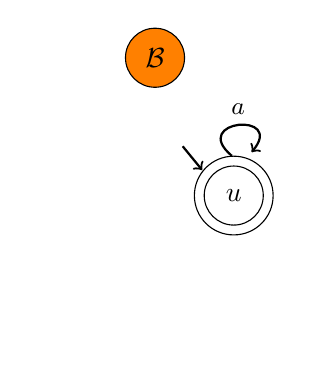
\begin{tikzpicture}
[
  scale=0.5
]

\node (start) at(-1,1) {};
\draw (2,8.5)[fill=orange] circle (0.75);
\draw (2,8.5) node {$\mathcal{B}$};

\draw (4,5) circle (1);
\draw (4,5) circle (0.75);
\draw (4,5) node {$u$};

\node (s) at (2.5,6.5) {};
\node (sx) at (3.4,5.4) {};

\node (x) at (4.2,5.8) {};
\node (x1) at (4.4,4.3) {};

\path[->,thick,every node/.style={font=\sffamily\small}]
  (x) edge [out=140, in=50, loop] node[above] {$a$} (x)

  (s) edge (sx);
\end{tikzpicture}

    \caption{The figure shows two NFA $\mathcal{A}$, $\mathcal{B}$ 
      which are used in example describing computation of a congruence closure in figure \ref{figHKCRew}}
		\label{figHKCex}
\end{center}
\end{figure}

\begin{figure}[bt]
  \begin{center}
    \begin{tikzpicture}[scale=0.12]
    \tikzstyle{every node}+=[inner sep=0pt]
    \draw (-20,0) node {\textit{\textcolor{Green}{$\{x,y\}$}}};
    \node (xy) at (-20,-2) {};  
    \draw (34,0) node {\textit{\textcolor{blue}{$\{u\}$}}};
    \node (u) at (32,-2) {};  

    \node (xyuU) at (-12,-8) {}; 
    \draw (-10,-10) node {\textit{\textcolor{Green}{$\{x,y,u\}$}}};
    \node (xyuP) at (-6,-12) {};

    \node (xuU) at (25,-8) {}; 
    \draw (22,-10) node {\textit{\textcolor{blue}{$\{x,u\}$}}};
    \node (xuP) at (20,-12) {}; 

    \node (xyzu) at (5,-18) {};
    \node (xyzu1) at (9,-18) {};
    \node (xyzu2) at (45,-18) {};
    \draw (7,-20) node {\textit{\textcolor{red}{$\{x,y,z,u\}$}}};

    
    \draw[->,thick,dashed] (xy) -- (xyuU);
    \draw[->,thick,dashed] (xyuP) -- (xyzu);
    \draw[->,thick,dashed] (u) -- (xuU);
    \draw[->,thick,dashed] (xuP) -- (xyzu1);
\end{tikzpicture}

    \caption{The figure (taken from \cite{popl13}) shows the deriving of the normal forms of the sets $\{x,y\}$ and $\{u\}$ using rewriting
      rules of the macrostates of a relation $R=\{(\{x\},\{u\}),(\{y,z\},\{u\})\}$.}
    \label{figHKCRew}
  \end{center}
\end{figure}

Problem of this approach is that we do not know which rules of relation $R$ to use, in which order to use the 
and each rule can be used only once for computing a normal form. 
Due this conditions the time complexity for finding one rule is in the worst case $rn$, where $r=|R|$ and $n=|Q|$ where $Q$ is a set of states of a NFA.
The whole derivation of the normal set is bounded by complexity $r^2 n$ because we apply maximally $r$ rules \cite{popl13}.

\subsubsection{Optimization for Inclusion Checking}
\label{congrOpt}
Since the algorithm based on bisimulation up to congruence is primarily used for checking equivalence of NFA it is possible to make some simplifications for
checking inclusion. An optimization is possible in checking whether macrostate $(X,Y)$ is in congruence closure of a relation $R$ of the visited
product states. The optimization
is based on the fact that when one checks inclusion between NFA $\mathcal{A}$ and $\mathcal{B}$ it is done by checking if $\mathcal{A}\cup\mathcal{B}=
\mathcal{B}$ so in all product states $(X,Y)$ is $X$ set of states of NFA $\mathcal{A}\cup\mathcal{B}$ and $Y$ set of states of NFA $\mathcal{B}$. Since the
states of $\mathcal{B}$ are already in macrostate $X$ it is useful to use the rewriting rules only in following form \cite{popl13}:
\begin{center}
$Y\rightarrow X\cup Y$
\end{center}
During checking inclusion of two NFA is not also necessary to achieve $X{\downarrow_R}=Y{\downarrow_R}$ to prove that $(X,Y)\in c(R)$ 
but just $X \subseteq Y{\downarrow_R}$ to prove that $(X\cup Y,Y)\in c(R)$ \cite{popl13}.

As an example is given computation of congruence closure during checking inclusion between NFA $\mathcal{A}$ and $\mathcal{B}$ (both are on the figure 
\ref{figHKCex}). Let have a relation of visited product states $R=\{(\{x,u\},\{u\}),(\{y,z,u\},\{u\})\}$ and newly generated product state $(\{x,y,u\},\{u\})$. The
derivation of the normal form of the set $\{u\}$ is shown on the figure \ref{figHKCRewO}. 
The normal form of the set $\{u\}$ is derived in two steps, first is applied rule $\{u\}\rightarrow\{x,u\}$ (based on $(\{x,u\},\{u\})\in R$) 
so we get a set $\{x,u\}$. Then rule $\{u\}\rightarrow\{y,z,u\}$ (based on $(\{y,z,u\},u)$) is used and the finally derived normal form is set $(\{x,y,z,u\})$ 
and because the set $\{x,y,u\}$ is subset of the derived set it holds that $(\{x,y,u\},\{u\})\in c(R)$.

\begin{figure}[bt]
  \begin{center}
    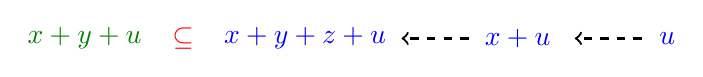
\begin{tikzpicture}[scale=0.1]
  \tikzstyle{every node}+=[inner sep=0pt]
  \draw (-30,0) node {\textit{\textcolor{Green}{$x+y+u$}}};
  \node (xy) at (-10,0) {};  
  \draw (-17.5,0) node {\textcolor{red}{$\subseteq$}};
  \draw (-2,0) node {\textit{\textcolor{blue}{$x+y+z+u$}}};
  \node (xmax) at (10,0) {};  
  \node (x+uP) at (19,0) {};  
  \draw (25,0) node {\textit{\textcolor{blue}{$x+u$}}};
  \node (x+u) at (32,0) {};  
  \draw (44,0) node {\textit{\textcolor{blue}{$u$}}};
  \node (u) at (41,0) {};  
  
  \draw[->,thick,dashed] (u) -- (x+u) ;
  \draw[->,thick,dashed] (x+uP) -- (xmax) ;
\end{tikzpicture}

    \caption{The figure shows the deriving of the normal form the set $\{u\}$ using rewriting
      rules of the elements of a relation $R=\{(\{x,u\},\{u\}),(\{y,z,u\},\{u\})\}$.}
    \label{figHKCRewO}
  \end{center}
\end{figure}

\chapter{Existing Finite Automata Libraries and the VATA Library} 
\label{libraries}
There are many different libraries for finite automata. These libraries have been created for various purposes and 
are implemented in different languages. 
At this chapter, some libraries will be described. Described libraries are just examples which represents typical disadvantages of existing libraries like
classical approach for language inclusion testing which needs the determinisation of finite automaton. 

At the second part of this chapter, VATA library for \emph{tree} automata will be introduced. 
Library design will be briefly described and also the operations for tree
automata and the plans for an extension of VATA library.

\section{Existing Finite Automata Libraries}
\label{existinglibraries}
\subsection{dk.brics.automaton}
\label{brics}
\emph{dk.brics.automaton} is an established Java package available under the BSD license. The latest version of this library (1.11-8) 
was released on September 7th, 2011.
Library can be downloaded and more information are on its webpage \cite{brics}. 

Library can use as input regular expression created by the Java \emph{RegEx} class.
It supports manipulation with NFA and DFA. Basic operation like union,
intersection, complementation or run of automaton on the given word etc., are available.

Test of language inclusion is also supported but if the input automaton is NFA, it needs to be converted to DFA. 
This is made by \emph{subset construction} approach which causes state explosion.

\emph{dk.brics.automaton} was ported to another two languages in two different libraries, which will be described next.

\subsubsection{libfa}
\emph{libfa} is a C library being part of \emph{Augeas} tool. 
Library is licensed under the LGPL, version 2 or later. It also support both versions of finite automata, NFA and DFA. 
Regular expressions could serve like input again.
libfa can be found and downloaded on it webpage \cite{libfa}.
libfa has no explicit operation for inclusion checking, but has the operations for intersection and complement of automata
which can serve for the inclusion checking.
Main disadvantage of libfa is again the need of the explicit determinisation during inclusion checking.

\subsubsection{Fare}
\emph{Fare} is a library, which brings dk.brics.automaton from Java to .NET. 
This library has the same characteristics as dk.brics.automaton or libfa and disadvantage in need of determinisation is still here. 
Fare can be found on its webpage \cite{fare}.

\subsection{The RWHT FSA toolkit}
The \emph{RWHT FSA} is a toolkit for manipulating finite automata described in \cite{kanthakN04}. 
The latest version is 0.9.4 from year 2005. The toolkit is written in C++
and available under its special license, derived from Q Public License v1.0 and the Qt Non-Commercial License v1.0. Library can be downloaded from \cite{rwth}. 

The RWHT FSA does not support only the classical finite automata, but also automata with weighted transitions so the toolkit has wider range of application.
The toolkit implements some techniques for better computation efficiency. E.g., it supports on-demand computation technique for operations over finite automata 
so not all computations are evaluated immediately but some are not computed until their results are really
needed. Usage of this technique leads to better memory efficiency. 

The RWHT FSA toolkit does not support language inclusion checking explicitly, but contains operations for intersection, complement and
determinisation which can be exploited for testing inclusion. This brings again the disadvantage of a state explosion during 
the explicit determinization. 

\subsection{Implementation of the State-of-the-art Algorithms}
There have been recently introduced some new efficient algorithms for inclusion checking 
which are dealing with problem of a state explosion because they avoid the explicit determinization of a finite automaton. These 
algorithms have been described in section \ref{chapInclusion}.
All of the mentioned state-of-the-art algorithms were implemented in OCaml language for testing and evaluation purposes.

The algorithms using the antichains are possible to use not only for finite automata but also for tree automata(\cite{cav06,tacas10}). 
The algorithms for tree automata are provided by the VATA library which is implemented in C++ what brings the greater efficiency compared to OCaml implementation. 
A description of this library will be placed in next section.
Despite the fact that a C++ implementation could be more efficient then OCaml  implementation, there is currently 
no library or toolkit similar to VATA library providing efficient implementation of these algorithms for language inclusion checking over NFA.


\begin{comment}
For finite automata manipulation exists many different libraries. Libraries have different purposes and are implemented in different languages, 
e.g. established package of Java \emph{dk.brics.automaton} \cite{brics}, \cite{tacas10}, which is also reimplemented for C in \emph{libfa} \cite{libfa} 
and for C\# in \emph{Fare} \cite{fare}. Another libraries are \emph{The RWTH FSA toolkit} \cite{rwth} in C++, which also supports weighted automata, or
\emph{FSA Utilities toolbox} \cite{fsaprolog} in Prolog.

This is not definitely complete enumeration of finite automata libraries, but just few examples. Their main problem is that they do not contain 
the efficient inclusion testing. On the other side, new efficient algorithms introduced in \cite{cav06,tacas10} and in \cite{popl13} have been for finite automata
implemented only in OCaml and implementation in C++ could be much more efficient.

Because of these reasons, algorithms for finite automata manipulation will be implemented as extension of VATA (library for tree automata manipulation) in C++.
\end{comment}

\section{VATA library}
\label{VATA}
VATA is a highly efficient open source library for \emph{nondeterministic tree} automata licensed under GPL, version 3. 
Main application of VATA is formal verification \cite{libvata}.
VATA library is implemented in C++ and uses the Boost C++ library. The library can be downloaded from its website 
\footnote{\url{http://www.fit.vutbr.cz/research/groups/verifit/tools/libvata/}}.  

\subsection{Design}
\label{sectionDesignVata}
VATA provides two kind of encoding for tree automata -- Explicit Encoding (top-down) and Semi-symbolic encoding (top-down and bottom-up). The main difference
between encoding is
in data structure for storing transition of tree automata. Semi-symbolic encoding is primary for automata with large alphabets. 

The main idea of the design of VATA library is show on the image \ref{picVataDesign} and here is also brief description of it. 
An input automaton is processed by one of the parsers (currently
is implemented only Timbuk format parser). A result of parsing is a data structure with the general information about automaton (the data structure stores a list
of transitions of a given automaton, its final states etc.). The main program choose one of the internal encodings of the automaton. The encodings
differs by a data structure they use for a representation of the automaton. Each encoding also provides the functions for transformation of the automaton 
from the data structure given by parser to the data structure used by chosen encoding. The encodings also implements
the operations over automata. When the automaton is processed it is often dumped to output format. 
This is done by one of the serializers (currently there is implemented only the Timbuk format serializer too) 
which takes as input the same data structure which uses parser.

As you can see on the figure \ref{picVataDesign}, the VATA library is written in a modular way, so it is easy to make an extension for finite automata. 
Thanks to the modularity, any new encoding can share other parts of library such as parser or serializer \cite{libvata}. 
The VATA library also provides a command line interface which is shared by different encodings.

\begin{figure}[bt]
\begin{center}
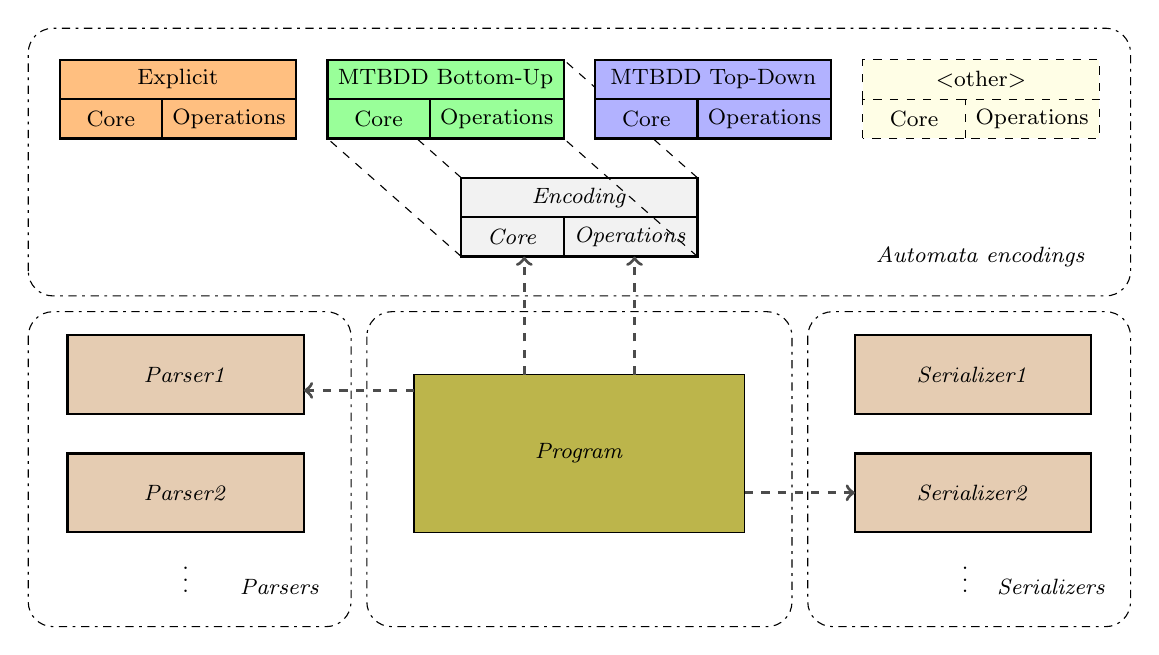
\begin{tikzpicture}
[
  scale=1,
  transform shape,
	gen/.style={thick,fill=gray!10},
	expl/.style={thick,fill=orange!50},
	bu/.style={thick,fill=green!40},
	td/.style={thick,fill=blue!30},
	other/.style={fill=yellow!10,dashed}
]
\tikzstyle{every node}=[font=\footnotesize]


% encodings
\draw[dashed] (0,1) -- (-1.7,2.5);
\draw[dashed] (0,0) -- (-1.7,1.5);
\draw[dashed] (3,1) -- (1.3,2.5);

\draw (0,0.5) rectangle +(3, 0.5) [gen] node[midway] {\textit{Encoding}};
\draw (0,0) rectangle +(1.3, 0.5) [gen] node[midway] {\textit{Core}};
\draw (1.3,0) rectangle +(1.7, 0.5) [gen] node[midway] {\textit{Operations}};

\draw (-5.1,2) rectangle +(3, 0.5) [expl] node[midway] {Explicit};
\draw (-5.1,1.5) rectangle +(1.3, 0.5) [expl] node[midway] {Core};
\draw (-3.8,1.5) rectangle +(1.7, 0.5) [expl] node[midway] {Operations};

\draw (-1.7,2) rectangle +(3, 0.5) [bu] node[midway] {MTBDD Bottom-Up};
\draw (-1.7,1.5) rectangle +(1.3, 0.5) [bu] node[midway] {Core};
\draw (-0.4,1.5) rectangle +(1.7, 0.5) [bu] node[midway] {Operations};

\draw (1.7,2) rectangle +(3, 0.5) [td] node[midway] {MTBDD Top-Down};
\draw (1.7,1.5) rectangle +(1.3, 0.5) [td] node[midway] {Core};
\draw (3.0,1.5) rectangle +(1.7, 0.5) [td] node[midway] {Operations};

\draw (5.1,2) rectangle +(3, 0.5) [other] node[midway] {$<$other$>$};
\draw (5.1,1.5) rectangle +(1.3, 0.5) [other] node[midway] {Core};
\draw (6.4,1.5) rectangle +(1.7, 0.5) [other] node[midway] {Operations};

\draw[dashed] (3,0) -- (1.3,1.5);

\draw[rounded corners=9,dash pattern=on 3pt off 2pt on 1pt off 2pt] (-5.5,-0.5) rectangle +(14,3.4);

\draw (6.6,0) node {\textit{Automata encodings}};


% parsers
\draw (-5,-2) rectangle +(3, 1) [gen,fill=brown!40] node[midway] (parser1) {\textit{Parser1}};
\draw (-5,-3.5) rectangle +(3, 1) [gen,fill=brown!40] node[midway] {\textit{Parser2}};
\draw (-3.5,-4) node {$\vdots$};

\draw[rounded corners=9,dash pattern=on 3pt off 2pt on 1pt off 2pt] (-5.5,-0.7) rectangle +(4.1,-4);
\draw (-2.3,-4.2) node {\textit{Parsers}};

% serializers
\draw (5,-2) rectangle +(3, 1) [gen,fill=brown!40] node[midway] {\textit{Serializer1}};
\draw (5,-3.5) rectangle +(3, 1) [gen,fill=brown!40] node[midway] {\textit{Serializer2}};
\draw (6.4,-4) node {$\vdots$};

\draw[rounded corners=9,dash pattern=on 3pt off 2pt on 1pt off 2pt] (4.4,-0.7) rectangle +(4.1,-4);
\draw (7.5,-4.2) node {\textit{Serializers}};

% program
\draw[rounded corners=9,dash pattern=on 3pt off 2pt on 1pt off 2pt] (-1.2,-0.7) rectangle +(5.4,-4);

\draw[fill=olive!60] (-0.6,-1.5) rectangle (3.6,-3.5) node[midway] {\textit{Program}};

\draw[very thick,dashed,->,black!70] (-0.6,-1.7) -- (-2,-1.7);
\draw[very thick,dashed,->,black!70] (3.6,-3) -- (5,-3);
\draw[very thick,dashed,->,black!70] (0.8,-1.5) -- (0.8,0);
\draw[very thick,dashed,->,black!70] (2.2,-1.5) -- (2.2,0);

\end{tikzpicture}

		\caption{The VATA library design. The image is taken from \cite{libvata}}.
		\label{picVataDesign}
\end{center}
\end{figure}

%%TODO: Vic se rozkecat o kodovanich
\subsubsection{Explicit Encoding}
\label{sectionExplicitEnc}
The explicit encoding supports storing the transitions in top-down direction (transitions are in form $q \xrightarrow{a} (q_1,...,q_n)$). The transitions
are stored in a \emph{hierarchical data structure based on hash tables}. First level of the data structure is hash table
that maps the states to \emph{transition cluster}. This clusters are also look-up tables and maps symbols of an input alphabet
to a set of pointers (stored as \emph{red-black tree}) to tuples of states. Storing tuples of states can be very memory demanding, so each tuple is stored
only once and is pointed by different transitions. 
Inserting new transition to this structure requires a constant number of steps (exception is the worst case scenario)
\cite{libvata}. This data structure can be seen on figure \ref{figExplicitTreeDataStr}.

\begin{figure}[bt]
\begin{center}
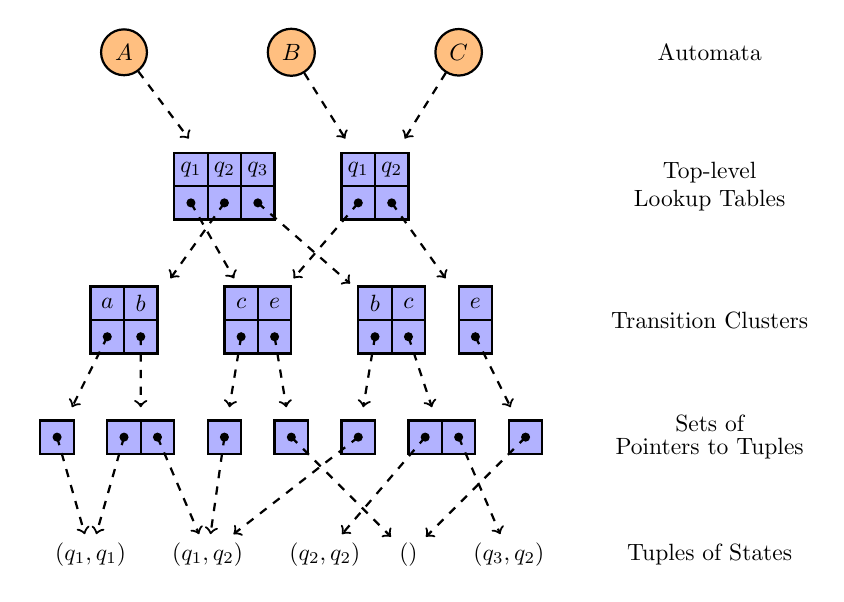
\begin{tikzpicture}
[
  scale=0.85,
  transform shape,
	gen/.style={thick,fill=gray!10},
	expl/.style={thick,fill=orange!50},
	bu/.style={thick,fill=green!40},
	td/.style={thick,fill=blue!30},
	other/.style={fill=yellow!10,dashed}
]

\node at(10,2) {Automata};

\node[expl,circle,draw] (aA) at(1.25,2) {\textit{$A$}};
\node[expl,circle,draw] (aB) at(3.75,2) {\textit{$B$}};
\node[expl,circle,draw] (aC) at(6.25,2) {\textit{$C$}};


\node at(10,0) {\shortstack{Top-level\\ Lookup Tables}};

\node[minimum size=40pt](table1) at (2.75,0) {};
\draw (2,0) rectangle +(0.5, .5) [td] node[midway] {\textit{$q_1$}};
\draw (2,-.5) rectangle +(0.5, .5) [td] node[midway] {};
\draw (2.5,0) rectangle +(0.5, .5) [td] node[midway] {\textit{$q_2$}};
\draw (2.5,-.5) rectangle +(0.5, .5) [td] node[midway] {};
\draw (3,0) rectangle +(0.5, .5) [td] node[midway] {\textit{$q_3$}};
\draw (3,-.5) rectangle +(0.5, .5) [td] node[midway] {};

\node[minimum size=40pt](table2) at (5,0) {};
\draw (4.5,0) rectangle +(0.5, .5) [td] node[midway] {\textit{$q_1$}};
\draw (4.5,-.5) rectangle +(0.5, .5) [td] node[midway] {};
\draw (5,0) rectangle +(0.5, .5) [td] node[midway] {\textit{$q_2$}};
\draw (5,-.5) rectangle +(0.5, .5) [td] node[midway] {};


\draw[->,thick,dashed] (aA) -- (table1);
\draw[->,thick,dashed] (aB) -- (table2);
\draw[->,thick,dashed] (aC) -- (table2);


\node at(10,-2) {Transition Clusters};

\node[minimum size=35](cluster1) at (1.5,-2) {};
\draw (0.75,-2) rectangle +(0.5, .5) [td] node[midway] {\textit{$a$}};
\draw (0.75,-2.5) rectangle +(0.5, .5) [td] node[midway] {};
\draw (1.25,-2) rectangle +(0.5, .5) [td] node[midway] {\textit{$b$}};
\draw (1.25,-2.5) rectangle +(0.5, .5) [td] node[midway] {};

\node[minimum size=35pt](cluster2) at (3.25,-2) {};
\draw (2.75,-2) rectangle +(0.5, .5) [td] node[midway] {\textit{$c$}};
\draw (2.75,-2.5) rectangle +(0.5, .5) [td] node[midway] {};
\draw (3.25,-2) rectangle +(0.5, .5) [td] node[midway] {\textit{$e$}};
\draw (3.25,-2.5) rectangle +(0.5, .5) [td] node[midway] {};

\node[minimum size=35pt](cluster3) at (5.25,-2) {};
\draw (4.75,-2) rectangle +(0.5, .5) [td] node[midway] {\textit{$b$}};
\draw (4.75,-2.5) rectangle +(0.5, .5) [td] node[midway] {};
\draw (5.25,-2) rectangle +(0.5, .5) [td] node[midway] {\textit{$c$}};
\draw (5.25,-2.5) rectangle +(0.5, .5) [td] node[midway] {};

\node[minimum size=35pt](cluster4) at (6.5,-2) {};
\draw (6.25,-2) rectangle +(0.5, .5) [td] node[midway] {\textit{$e$}};
\draw (6.25,-2.5) rectangle +(0.5, .5) [td] node[midway] {};


\draw[thick,fill=black] (2.25,-0.25) circle (0.5mm);
\draw[->,thick,dashed] (2.25,-.25) -- (cluster2);

\draw[thick,fill=black] (2.75,-0.25) circle (0.5mm);
\draw[->,thick,dashed] (2.75,-.25) -- (cluster1);

\draw[thick,fill=black] (3.25,-0.25) circle (0.5mm);
\draw[->,thick,dashed] (3.25,-.25) -- (cluster3);

\draw[thick,fill=black] (4.75,-0.25) circle (0.5mm);
\draw[->,thick,dashed] (4.75,-.25) -- (cluster2);

\draw[thick,fill=black] (5.25,-0.25) circle (0.5mm);
\draw[->,thick,dashed] (5.25,-.25) -- (cluster4);


\node at(10,-3.75) {\shortstack{Sets of\\ Pointers to Tuples}};

\node[minimum size=25pt](set1) at (0.25,-3.75) {};
\draw (0,-4) rectangle +(0.5, .5) [td] node[midway] {};

\node[minimum size=25pt](set2) at (1.5,-3.75) {};
\draw (1,-4) rectangle +(0.5, .5) [td] node[midway] {};
\draw (1.5,-4) rectangle +(0.5, .5) [td] node[midway] {};

\node[minimum size=25pt](set3) at (2.75,-3.75) {};
\draw (2.5,-4) rectangle +(0.5, .5) [td] node[midway] {};

\node[minimum size=25pt](set4) at (3.75,-3.75) {};
\draw (3.5,-4) rectangle +(0.5, .5) [td] node[midway] {};

\node[minimum size=25pt](set5) at (4.75,-3.75) {};
\draw (4.5,-4) rectangle +(0.5, .5) [td] node[midway] {};

\node[minimum size=25pt](set6) at (6,-3.75) {};
\draw (5.5,-4) rectangle +(0.5, .5) [td] node[midway] {};
\draw (6,-4) rectangle +(0.5, .5) [td] node[midway] {};

\node[minimum size=25pt](set7) at (7.25,-3.75) {};
\draw (7,-4) rectangle +(0.5, .5) [td] node[midway] {};


\draw[thick,fill=black] (1,-2.25) circle (0.5mm);
\draw[->,thick,dashed] (1,-2.25) -- (set1);

\draw[thick,fill=black] (1.5,-2.25) circle (0.5mm);
\draw[->,thick,dashed] (1.5,-2.25) -- (set2);

\draw[thick,fill=black] (3,-2.25) circle (0.5mm);
\draw[->,thick,dashed] (3,-2.25) -- (set3);

\draw[thick,fill=black] (3.5,-2.25) circle (0.5mm);
\draw[->,thick,dashed] (3.5,-2.25) -- (set4);

\draw[thick,fill=black] (5,-2.25) circle (0.5mm);
\draw[->,thick,dashed] (5,-2.25) -- (set5);

\draw[thick,fill=black] (5.5,-2.25) circle (0.5mm);
\draw[->,thick,dashed] (5.5,-2.25) -- (set6);

\draw[thick,fill=black] (6.5,-2.25) circle (0.5mm);
\draw[->,thick,dashed] (6.5,-2.25) -- (set7);


\node at(10,-5.5) {Tuples of States};

\node(tup1) at (0.75,-5.5) {$(q_1, q_1)$};
\node(tup2) at (2.5,-5.5) {$(q_1, q_2)$};
\node(tup3) at (4.25,-5.5) {$(q_2, q_2)$};
\node(tup4) at (7,-5.5) {$(q_3, q_2)$};
\node(tup5) at (5.5,-5.5) {$()$};

\draw[thick,fill=black] (0.25,-3.75) circle (0.5mm);
\draw[->,thick,dashed] (0.25,-3.75) -- (tup1);

\draw[thick,fill=black] (1.25,-3.75) circle (0.5mm);
\draw[->,thick,dashed] (1.25,-3.75) -- (tup1);

\draw[thick,fill=black] (1.75,-3.75) circle (0.5mm);
\draw[->,thick,dashed] (1.75,-3.75) -- (tup2);

\draw[thick,fill=black] (2.75,-3.75) circle (0.5mm);
\draw[->,thick,dashed] (2.75,-3.75) -- (tup2);

\draw[thick,fill=black] (3.75,-3.75) circle (0.5mm);
\draw[->,thick,dashed] (3.75,-3.75) -- (tup5);

\draw[thick,fill=black] (4.75,-3.75) circle (0.5mm);
\draw[->,thick,dashed] (4.75,-3.75) -- (tup2);

\draw[thick,fill=black] (5.75,-3.75) circle (0.5mm);
\draw[->,thick,dashed] (5.75,-3.75) -- (tup3);

\draw[thick,fill=black] (6.25,-3.75) circle (0.5mm);
\draw[->,thick,dashed] (6.25,-3.75) -- (tup4);

\draw[thick,fill=black] (7.25,-3.75) circle (0.5mm);
\draw[->,thick,dashed] (7.25,-3.75) -- (tup5);


\end{tikzpicture}

    \caption{The data structure for storing transitions of the tree automaton. There is a hash table (top-level look-up table) 
      which map a state to the pointer to another hash table (transition cluster). Transition cluster
      maps a symbols of input alphabet to the pointer to the set of pointers to the tuples of states.}
		\label{figExplicitTreeDataStr}
\end{center}
\end{figure}


For better performance is used \emph{copy-on-write} technique \cite{libvata}. The principle of this technique is 
that on copy of automaton is created just new pointer to transition table of original automaton and after adding a new state to one of the automaton 
is modified only part of the whole shared transition table. 

\subsubsection{Semi-symbolic Encoding}
Transition functions in semi-symbolic encoding are stored in \emph{multi-terminal binary decision diagrams} (MTBDD), which are extension of \emph{binary decision 
diagrams}. There are provided top-down (transitions are in form $q \xrightarrow{a} (q_1,...,q_n)$, for $a$ with arity $n$) 
and bottom-up (transitions are in form $(q_1,...,q_n)\xrightarrow{a}q$) representation of tree automata in semi-symbolic encoding. 
The specific part is the saving of symbols in MTBDD. In top-down encoding, the input
symbols are stored in MTBDD with their arity, because we need to be able to distinguish between two instances of same symbols with different arity.
In opposite case, bottom-up encoding does not need to store arity, because it is possible to get it from arity of tuple on left side of transition \cite{libvata}.

For purposes of VATA library was implemented new MTBDD package which improved the performance of library.

%TODO povypravaet o MTBDD package

\subsubsection{Operations}
There are supported basic operations over tree automata 
like union, intersection, elimination of unreachable states, but also some advance a algorithms for inclusion checking, 
computation of simulation relation, language preserving size reduction based on simulation equivalence. 

Optimized algorithms for inclusion testing \cite{cav06,tacas10} are implemented. The inclusion operation is implemented in more versions, so it is possible
to use only some heuristic and compare different results.

The efficiency of advanced operations does not come only from the usage of the state-of-the-art algorithms, 
but there are also some implementation optimization like \emph{copy-on-write}
principle for automata copying (briefly described in section \ref{sectionExplicitEnc}), buffering once computed clusters of transitions, etc. 
Other optimization could be found in exploitation of polymorphism using C++ function templates, instead of
virtual method because a call of virtual function leads to indirect function call using look-up in virtual-method table (because compiler does not know, which 
function will be called in runtime) what brings an overhead compared to classical direct 
function call and it also precludes compiler's optimizer to perform some operations \cite{libvata}. 
%TODO Moznost citatce 

More details about implementation optimization can be found in \cite{libvata}.

Especially advanced operations are able only for specific encoding. Some of operations implemented in VATA library and their supported encodings are in 
the table \ref{tabOp}.
\begin{savenotes}
\begin{table}[h]
	\begin{center}
		\catcode`\-=12
		\begin{tabular}{| l | c | c | c |} \hline
		& {\textbf{Explicit}} & \multicolumn{2}{|c|}{\textbf{Semi-symbolic}} \\ \cline{2-4}
		\textbf{Operation} & \textbf{top-down} & \textbf{bottom-up} & \textbf{top-down} \\ \hline
		Union & $+$ & $+$ & $+$ \\
		Intersection & $+$ & $+$ & $+$ \\
		Complement & $+$ & $+$ & $+$ \\
		Removing useless states & $+$ & $+$ & $+$ \\
		Removing unreachable states & $+$ & $+$ & $+$ \\
		Downward and Upward Simulation & $+$ & $-$ & $+$ \\
		Bottom-Up Inclusion  & $+$ & $+$ & $-$ \\ 
		Simulation over LTS\footnote{LTS -- Labeled Transitions System} & $+$ & $-$ & $-$ \\ \hline
		\end{tabular}
	\caption{Table shows which operations are supported for the tree automata in the encodings implemented in VATA library.}
	\label{tabOp}
	\end{center}
\end{table}
\end{savenotes}


\subsection{Extension for Finite Automata}
The purposes of the VATA library are similar as purposes of this work and because the VATA library is written in modular way, it is easy 
to extend it by another module, so it was decided not to create a brand new library but implement a new extension of VATA for finite automata.

The main goal is to provide efficient implementation of the operation for checking of the language inclusion using state-of-the-art algorithms. 
To be precise, VATA library could be already used for finite automata which can be represented by one dimensional
tree automata. But the VATA library data structures for manipulating tree automata are designated for more complex data structures
and new special implementation for finite automata will be definitely more efficient. 
Not only the inclusion checking algorithms will be implemented but also the algorithms for basic operations like union, intersection, removing unreachable or 
useless states. The new extension will implement only the explicit encoding of finite automata. 
The extension will use some already implemented features of the VATA library like parser and serializer or computation of simulation over states of an automaton.

\chapter{Design}
\label{design}
This chapter is primarily about design of the newly created extension of VATA library for finite automata. 
At first, the data structures used for storing a finite automaton will be described then a principle of translation of the states and the symbols of a NFA 
to internal representation. The choice of an input format and its modification are justified.  
The algorithms for basic operations over NFA like union, intersection or removing unreachable states, etc., are given at the end of the chapter.

\section{Data Structures for Explicit Encoding of Finite Automata}
The encodings for tree automata used in VATA library differ mainly in a data structure used for storing transitions of tree automata. The explicit encoding
for finite automata is defined by a data structure used for storing the transitions too. 
This data structure is also crucial performance of the algorithms so it is important to good analyze and design it. 

\label{data structure explicit}
\subsection{Analysis}
\label{analysis}
A NFA is defined by set of its states, its start and final states (which are subset of all states of the NFA) and also its
transitions and the input alphabet (a formal definition is given in section \ref{defNFA}). 
One needs to keep information about sets of start and final states to be able to distinguish
between them and the other states. But it is not necessary to store the whole set of states alone because states are used only within transitions. 
This also holds for an input alphabet of the NFA. 

The transitions keep the most information about a NFA and are also often used
during the operations over NFA, so the the performance of these operations strongly depend on the efficiency of data structure for a set of transitions. 
For example, in many operations over NFA one wants to get all transitions for a given state and a given alphabet symbol and it is important for 
the efficiency of the algorithms to get those transitions in as few steps as possible. The similar needs are in the case
of tree automata when it is not necessary to hold the whole set of the states but it is important to have an efficient data structure for representing 
transitions of the tree automata.

The data structure used for storing transitions of a tree automaton in the VATA library was described earlier in section \ref{sectionExplicitEnc} and can be seen
on the figure \ref{figExplicitTreeDataStr}. The evaluation of the VATA library \cite{libvata} proves the efficiency of this data structure so it was
decided to modify it and implement the modification in the extension of the VATA library for finite automata.

\subsection{Design of Data Structure for Transitions of NFA}
A data structure for storing transitions of a NFA is based on hash tables. The first hash table (top-level hash table) maps a given state to the pointer to
a transition cluster. The transition cluster is another hash table which maps a given symbol of the input alphabet to a set of states accessible from
the given state under the given symbol. 
Described data structure is on the figure \ref{figExplicitFADataStr}.

The data structure for storing of the finite automata transitions is simplification of the data structure for the tree automata. Since a tree automaton's
transition has following form: $q \xrightarrow{a} (q_1,\ldots,q_n)$ where $q,q_1\ldots q_n$ are states of the tree automaton and $a$ is the symbol of 
the input alphabet of the tree automaton and a finite automaton has transition in form: $q_1 \xrightarrow{a} q_2$ 
where $q_1,q_2$ are states of the finite automaton and $a$ is its symbol, the simplification of data structure is possible because 
the tree version has to store the whole tuples. These tuples can be very large and it is more efficient to store them only once in a cache and 
in the data structure for transitions work only with pointer to a tuple instead of the tuple alone. 

In case of finite automata this advantage disappears because there are no tuples of state but only states alone and keeping pointer to one state will not 
bring any memory efficiency (a size of a pointer to a state and the state represented by integer alone is quite similar). This causes that for the data structure 
for finite automata is not needed to use anything such as a set of pointers to tuples, but could be directly used a set of states instead of
a set of pointers. The set of states would be pointed from transition cluster and would contain all states accessible from a given state under a 
certain symbol of the input alphabet.

But there is possible another simplification. The set of states does not need to be in a special set pointed by transition cluster but can be integrated
to the transition cluster. When this optimization is applied, transition cluster maps symbol directly to the set of states accessible under this symbol.

The mentioned optimization enables simplification from the four levels of data structure for tree automata to the two levels data structure used for finite
automata what brings simpler and more efficient manipulation with these data structure. A comparison of data structure for the finite automata and 
the tree automata can be seen on the figures \ref{figExplicitFADataStr} and figure \ref{figExplicitTreeDataStr}.

This data structure apply also the copy-on-write principle for better memory efficiency so the look-up tables and 
the transition clusters are shared among NFA when they are same and
a new look-up table and a transition is created only when a new item is inserted to the one of the automata. For example, NFA $\mathcal{A}$ and NFA $\mathcal{B}$
from the figure \ref{figExplicitFADataStr} are sharing the same data structure.

Let give the examples for searching and inserting a transition to this data structure for the NFA on the figure \ref{figExplicitFADataStr}. 
If one wants to find all accessible states for state $q_1$ and symbol $a$ in a NFA $\mathcal{A}$
so in the top-level look-up is $q1$ mapped to the pointer to transition cluster. In this
transition cluster is symbol $a$ mapped to the set of states (in this case ($\{q_1,q_2\}$)) which are accessible from $q_1$ under $a$.
If one wants to insert a new transition $q_3 \xrightarrow{e} q_2$ to a NFA $\mathcal{C}$, the look-up table pointed by automaton $\mathcal{C}$ is duplicated 
and a state $q_3$ is inserted to it. The NFA $\mathcal{C}$ now points to that newly duplicated look-up table. State $q_3$ is in this look-up table 
mapped to pointer to the newly created transition cluster. 
Symbol $e$ is inserted to this new transition cluster and mapped to the set of state which contains just state $q_2$.

\begin{figure}[bt]
\begin{center}
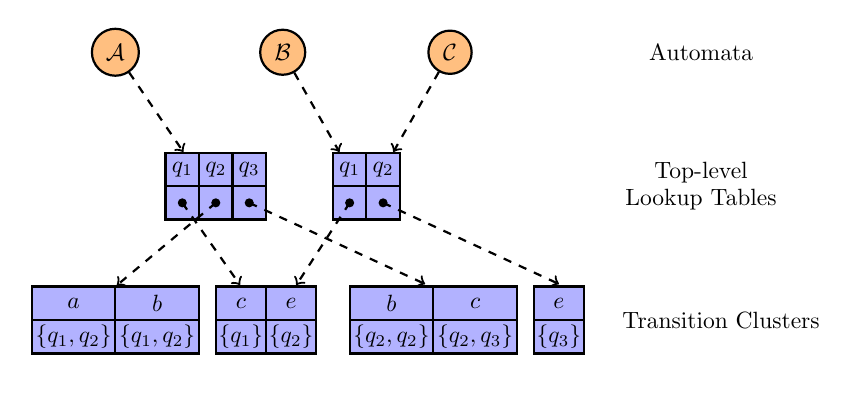
\begin{tikzpicture}
[
  scale=0.85,
  transform shape,
	gen/.style={thick,fill=gray!10},
	expl/.style={thick,fill=orange!50},
	bu/.style={thick,fill=green!40},
	td/.style={thick,fill=blue!30},
	other/.style={fill=yellow!10,dashed}
]

\node at(10,2) {Automata};

\node[expl,circle,draw] (aA) at(1.25,2) {\textit{$\mathcal{A}$}};
\node[expl,circle,draw] (aB) at(3.75,2) {\textit{$\mathcal{B}$}};
\node[expl,circle,draw] (aC) at(6.25,2) {\textit{$\mathcal{C}$}};


\node at(10,0) {\shortstack{Top-level\\ Lookup Tables}};

\node[minimum size=40pt](table1) at (2.75,-0.2) {};
\draw (2,0) rectangle +(0.5, .5) [td] node[midway] {\textit{$q_1$}};
\draw (2,-.5) rectangle +(0.5, .5) [td] node[midway] {};
\draw (2.5,0) rectangle +(0.5, .5) [td] node[midway] {\textit{$q_2$}};
\draw (2.5,-.5) rectangle +(0.5, .5) [td] node[midway] {};
\draw (3,0) rectangle +(0.5, .5) [td] node[midway] {\textit{$q_3$}};
\draw (3,-.5) rectangle +(0.5, .5) [td] node[midway] {};

\node[minimum size=40pt](table2) at (5,-0.2) {};
\draw (4.5,0) rectangle +(0.5, .5) [td] node[midway] {\textit{$q_1$}};
\draw (4.5,-.5) rectangle +(0.5, .5) [td] node[midway] {};
\draw (5,0) rectangle +(0.5, .5) [td] node[midway] {\textit{$q_2$}};
\draw (5,-.5) rectangle +(0.5, .5) [td] node[midway] {};


\draw[->,thick,dashed] (aA) -- (table1);
\draw[->,thick,dashed] (aB) -- (table2);
\draw[->,thick,dashed] (aC) -- (table2);


\node at(10.3,-2) {Transition Clusters};

\node[minimum size=35](cluster1) at (0.65,-2) {};
\draw (0.00,-2) rectangle +(1.25, .5) [td] node[midway] {\textit{$a$}};
\draw (0.00,-2.5) rectangle +(1.25, .5) [td] node[midway] {\textit{$\{q_1,q_2\}$}};
\draw (1.25,-2) rectangle +(1.25, .5) [td] node[midway] {\textit{$b$}};
\draw (1.25,-2.5) rectangle +(1.25, .5) [td] node[midway] {\textit{$\{q_1,q_2\}$}};

\node[minimum size=35pt](cluster2) at (3.55,-2.1) {};
\draw (2.75,-2) rectangle +(0.75, .5) [td] node[midway] {\textit{$c$}};
\draw (2.75,-2.5) rectangle +(0.75, .5) [td] node[midway] {\textit{$\{q_1\}$}};
\draw (3.5,-2) rectangle +(0.75, .5) [td] node[midway] {\textit{$e$}};
\draw (3.5,-2.5) rectangle +(0.75, .5) [td] node[midway] {\textit{$\{q_2\}$}};

\node[minimum size=35pt](cluster3) at (6.5,-1.75) {};
\draw (4.75,-2) rectangle +(1.25, .5) [td] node[midway] {\textit{$b$}};
\draw (4.75,-2.5) rectangle +(1.25, .5) [td] node[midway] {\textit{$\{q_2,q_2\}$}};
\draw (6.0,-2) rectangle +(1.25, .5) [td] node[midway] {\textit{$c$}};
\draw (6.0,-2.5) rectangle +(1.25, .5) [td] node[midway] {\textit{$\{q_2,q_3\}$}};

\node[minimum size=35pt](cluster4) at (8.5,-1.75) {};
\draw (7.5,-2) rectangle +(0.75, .5) [td] node[midway] {\textit{$e$}};
\draw (7.5,-2.5) rectangle +(0.75, .5) [td] node[midway] {\textit{$\{q_3\}$}};


\draw[thick,fill=black] (2.25,-0.25) circle (0.5mm);
\draw[->,thick,dashed] (2.25,-.25) -- (cluster2);

\draw[thick,fill=black] (2.75,-0.25) circle (0.5mm);
\draw[->,thick,dashed] (2.75,-.25) -- (cluster1);

\draw[thick,fill=black] (3.25,-0.25) circle (0.5mm);
\draw[->,thick,dashed] (3.25,-.25) -- (cluster3);

\draw[thick,fill=black] (4.75,-0.25) circle (0.5mm);
\draw[->,thick,dashed] (4.75,-.25) -- (cluster2);

\draw[thick,fill=black] (5.25,-0.25) circle (0.5mm);
\draw[->,thick,dashed] (5.25,-.25) -- (cluster4);
\end{tikzpicture}

    \caption{The data structure for storing transition of an finite automaton. There is a hash table (top-level look-up table) 
      which map a state of a FA to the pointer to another hash table (transition cluster). Transition cluster maps a symbol of the input alphabet
      to a set of states.}
		\label{figExplicitFADataStr}
\end{center}
\end{figure}

\section{Data Structure for Start and Final States}
As it was mentioned in previous section \ref{analysis} it is necessary to keep start and final states in the special sets to 
be able distinguish between them and the others states of an automaton. This is also main usage of these sets during operations 
over finite automata so there is no need to create special data structure and unordered set is efficient enough for this purposes.

\section{Translation of the States and Symbols}
\label{sectionTranslate}
An automaton is always parsed and converted to the intern representation from its input format. 
The conversion to the internal representation is based on mapping states from an input type (e.g. text description of the automaton) 
to the integers. This principle is also applied for symbols of the input alphabet. 
Mechanism of translation is illustrated by figure \ref{figExplicitFATransl}. 
The mechanism brings better efficiency for manipulation with states and symbols
during the operations. It also provides unification of all input forms to the one internal representation. 

Processing of some operations (e.g., union) can causes reindexing of the states what means that the integers 
which represents a state is changed. When the integer is changed an old value is mapped to a new one by a hash table what keeps 
relation between a original input value and the new integer value.

When the operations over a NFA are performed the NFA is often serialized back to the input format. The result 
automaton's states and symbols are mapped back to the input notation using hash tables where has been the mapping stored. This
principle brings more readable output of serialization because the original notation is kept.

\begin{figure}[bt]
\begin{center}
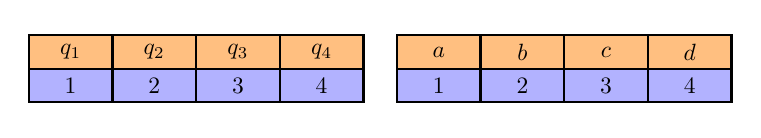
\begin{tikzpicture}
[
  scale=0.85,
  transform shape,
	gen/.style={thick,fill=gray!10},
	expl/.style={thick,fill=orange!50},
	bu/.style={thick,fill=green!40},
	td/.style={thick,fill=blue!30},
	other/.style={fill=yellow!10,dashed}
]

\node[minimum size=35](states) at (0.65,-2) {};
\draw (0.00,-2) rectangle +(1.25, .5) [expl] node[midway] {\textit{$q_1$}};
\draw (0.00,-2.5) rectangle +(1.25, .5) [td] node[midway] {\textit{$1$}};
\draw (1.25,-2) rectangle +(1.25, .5) [expl] node[midway] {\textit{$q_2$}};
\draw (1.25,-2.5) rectangle +(1.25, .5) [td] node[midway] {\textit{$2$}};
\draw (2.5,-2) rectangle +(1.25, .5) [expl] node[midway] {\textit{$q_3$}};
\draw (2.5,-2.5) rectangle +(1.25, .5) [td] node[midway] {\textit{$3$}};
\draw (3.75,-2) rectangle +(1.25, .5) [expl] node[midway] {\textit{$q_4$}};
\draw (3.75,-2.5) rectangle +(1.25, .5) [td] node[midway] {\textit{$4$}};

\node[minimum size=35](syms) at (0.65,-2) {};
\draw (5.5,-2) rectangle +(1.25, .5) [expl] node[midway] {\textit{$a$}};
\draw (5.5,-2.5) rectangle +(1.25, .5) [td] node[midway] {\textit{$1$}};
\draw (6.75,-2) rectangle +(1.25, .5) [expl] node[midway] {\textit{$b$}};
\draw (6.75,-2.5) rectangle +(1.25, .5) [td] node[midway] {\textit{$2$}};
\draw (8.0,-2) rectangle +(1.25, .5) [expl] node[midway] {\textit{$c$}};
\draw (8.0,-2.5) rectangle +(1.25, .5) [td] node[midway] {\textit{$3$}};
\draw (9.25,-2) rectangle +(1.25, .5) [expl] node[midway] {\textit{$d$}};
\draw (9.25,-2.5) rectangle +(1.25, .5) [td] node[midway] {\textit{$4$}};

\end{tikzpicture}

    \caption{The figure shows a principle of the translation of the input format to the internal representation by a hash table. 
      The states (the left hash table) or of the symbols (the right hash table) of a NFA are mapped from strings to the integers.}
		\label{figExplicitFATransl}
\end{center}
\end{figure}

\section{Usage of the Timbuk Format}
\label{usageTimbuk}
VATA library provides possibility to load a finite automaton from a text specification. 
The text specification of NFA has to have a standard format but there is no such format for the finite automata so it was chosen
the Timbuk format \cite{timbuk}. The Timbuk format is primarily used for description of the tree automata but can be also used for the finite automata
after some modifications. This format was also used as the input format of tree automata in VATA library.

Here is an example of an finite automaton defined by text description in the Timbuk format:\\
\texttt {
  \textbf{Ops} $a:1$ $x:0$\\
  \textbf{Automaton} foo\\
  \textbf{States} $s$ $p$ $q$ $f$\\
  \textbf{Final States} $f$\\
  \textbf{Transitions}\\
  \indent $x \rightarrow s$\\
  \indent $a(s) \rightarrow p$\\
  \indent $a(s) \rightarrow q$\\
  \indent $a(p) \rightarrow f$\\
  \indent $a(q) \rightarrow f$\\
}
On the first line of the specification in the Timbuk format
is specified that the automaton has only one symbol of the input alphabet $a$ with arity one (arity of the symbols of finite automata will
be always one). 
The need of specification of the arity of an input symbol is a lack which comes from the original purpose of the Timbuk format because it is necessary 
to give the arity of an symbol of an input alphabet of an tree automaton.

The second symbol $x$ with arity zero is not actually symbol of the input alphabet but is used for definition of the start states. The
start states are defined in section \emph{Transitions} by the transitions which has on the left side some symbol with zero arity and on the
right side of the transition is a start state. This is again disadvantage
of the Timbuk format because tree automata have no start states.

On the second line of the given example is name of the automaton (in our example is the name \emph{foo}). 
On the third line is a list of states of the automaton and on the fourth line is a list of final states of the automaton.

Then there is list of the transitions of the automaton. 
For example, the transition $s \xrightarrow{a} q$ is in the Timbuk format described like $a(s)\rightarrow q$.

\section{Algorithms for Basic Operations}
In this section are described algorithms used for implementation of the basic operations like union, intersection or removing useless states and others. 

\subsection{Union}
The union of two NFA $\mathcal{A}$ and $\mathcal{B}$ is described in section \ref{defAUnion} and
is done by following algorithm. First, a brand new automaton is created (this automaton
will be result of union). Sets of start and final states are copied to this automaton from both original automata. Then the all transitions from $\mathcal{A}$ and
$\mathcal{B}$ are added to the newly created automaton. What is the most important during these operations is reindexing of states (it is supposed
that the both automata have the same input alphabet so the symbols of it are not reindexed). The reindexing means that there is created index which maps
integer that represents a state in the input automaton to a new integer which will represent the same state in the automaton created by this union.

The reindexing of states is done because the same integer can be used for representing one state of a NFA $\mathcal{A}$ 
and also another state of a NFA $\mathcal{B}$ and it is important
to be able to distinguish between these two states in the result NFA. This technique also makes text output of serialization of the result automaton 
more readable because its states have the same names as it has in the input automata, only indices $1$ and $2$ are added to be able to 
distinguish between states of both automaton. E.g., a state $q$ of NFA $\mathcal{A}$ and a state $q$ of NFA $\mathcal{B}$ are in the result automaton denoted
as $q_1$ and $q_2$.

\subsubsection{Union of Disjunct States}
The special case of union of two NFA is union of disjunct states of these NFA. This is done by copying of the first NFA to the result automaton and then
the states (and transitions which contain these states) of the second NFA which are not already in the result NFA are copied to the result automaton.
No reindexing of states is done during this operation.

\subsection{Intersection}
The intersection of two NFA $\mathcal{A}=(Q_\mathcal{A},\Sigma,\delta_\mathcal{A},I_\mathcal{A},F_\mathcal{A})$
and $\mathcal{B}=(Q_\mathcal{A},\Sigma,\delta_\mathcal{B},I_\mathcal{B},F_\mathcal{B})$ is defined 
in preliminaries \ref{defAInter}. 
We define post-image of the product state $(p,q)\in \mathcal{A}\cap\mathcal{B}$ for a given symbol $a\in \Sigma$ by:\\
$Post_a((p,q)):=\{(p',q')\ |\ \exists a \in \Sigma: (p,a,p')\in \delta_a, (q,a,q')\in \delta_b\}$.\\
The algorithm for intersection is described by the algorithm \ref{algIntersection}.

The principle of this algorithm is following. The both input NFA are explored parallel and to the result automata are added product states. 
A product state consists two states each from different automaton which are accessible for the same string of input alphabet. 
The transitions of the result automaton contain also these product states.

\begin{algorithm}
	\label{algIntersection}
	\KwIn{NFA's $\mathcal{A}=(Q_\mathcal{A},\Sigma,\delta_\mathcal{A},I_\mathcal{A},F_\mathcal{A}),\ \mathcal{B}=(Q_\mathcal{A},\Sigma,
      \delta_\mathcal{B},I_\mathcal{B},F_\mathcal{B})$} 

  \KwOut{NFA $\mathcal{A}\cap\mathcal{B}$=($Q_{\mathcal{A}\cap\mathcal{B}},\Sigma,\delta_{\mathcal{A}\cap\mathcal{B}},
      I_{\mathcal{A}\cap\mathcal{B}},F_{\mathcal{A}\cap\mathcal{B}}$)}
  $Stack = \varnothing$\;

  \ForAll{$(p_\mathcal{A},p_\mathcal{B})\in I_\mathcal{A}\times I_\mathcal{B}$} {
    Add $(p_\mathcal{A},p_\mathcal{B})$ to $I_{\mathcal{A} \cap \mathcal{B}}$\;
    Push $(p_\mathcal{A},p_\mathcal{B})$ on $Stack$\; 
    \If{$(p_\mathcal{A} \in F_\mathcal{A} \wedge p_\mathcal{B} \in F_\mathcal{B})$} {
      Add $(p_\mathcal{A},p_\mathcal{B})$ to $F_{\mathcal{A}\cap\mathcal{B}}$
    }
  }
	
  \While{($Stack\neq \varnothing$)} {
			Pick and remove a product-state $(p_\mathcal{A},p_\mathcal{B})$ from $Stack$\;
			\ForAll{$(q_\mathcal{A},q_\mathcal{B})\in Post_a(p_\mathcal{A},p_\mathcal{B})$}{
        \If{$(q_\mathcal{A} \in F_\mathcal{A} \wedge q_\mathcal{B} \in F_\mathcal{B})$} {
          Add $(q_\mathcal{A},q_\mathcal{B})$ to $F_{\mathcal{A}\cap\mathcal{B}}$
        }
        Add $(p_\mathcal{A},p_\mathcal{B}) \xrightarrow{a} (q_\mathcal{A},q_\mathcal{B})$ to $\delta_{\mathcal{A}\cap\mathcal{B}}$\;
        Push $(q_\mathcal{A},q_\mathcal{B})$ on $Stack$\; 
      }
	 }
		\Return NFA $\mathcal{A}\cap\mathcal{B}$;
	\caption{Algorithm for intersection of NFA}
\end{algorithm}

\subsection{Reverse}
The reversion of an NFA $\mathcal{A}=(Q_\mathcal{A},\Sigma,\delta_\mathcal{A},I_\mathcal{A},F_\mathcal{A})$ is an NFA 
$\mathcal{A}_{rev}=(Q_{\mathcal{A}_{rev}},\Sigma,\delta_{\mathcal{A}_{rev}},I_{\mathcal{A}_{rev}},F_{\mathcal{A}_{rev}})$ 
which is created just by changing start state's set by final state's set what is done by
assigning $I_\mathcal{A}$ to $F_{\mathcal{A}_{rev}}$ and $F_\mathcal{A}$ to $I_{\mathcal{A}_{rev}}$ and reverting all transitions  so e.g., transition
$p\xrightarrow{x}q \in \delta_\mathcal{A}$ is added to $\delta_{\mathcal{A}_{rev}}$ in form $q\xrightarrow{a}p$. This principle is described by the algorithm
\ref{algRev}
\\

\begin{algorithm}[H]
	\label{algRev}
	\KwIn{NFA $\mathcal{A}=(Q_\mathcal{A},\Sigma,\delta_\mathcal{A},I_\mathcal{A},F_\mathcal{A})$} 

  \KwOut{NFA $\mathcal{A}_{rev}=(Q_{\mathcal{A}_{rev}},\Sigma,\delta_{\mathcal{A}_{rev}},I_{\mathcal{A}_{rev}},F_{\mathcal{A}_{rev}})$} 
  
  $F_{\mathcal{A}_{rev}}=I_\mathcal{A}$\; 
  $I_{\mathcal{A}_{rev}}=F_\mathcal{A}$\;

  \ForAll{$(p,a,q) \in \delta_{\mathcal{A}}$} {
    Add $(q,a,p)$ to $\delta_{\mathcal{A}_{rev}}$\;
  }
	\Return NFA $\mathcal{A}_{rev}$;
	\caption{Algorithm for reverting of an NFA}
\end{algorithm}

\subsection{Removing Unreachable States}
Let the NFA $\mathcal{B}$ be created by removing all unreachable states from an NFA $\mathcal{A}$ (an unreachable state of an NFA was defined in
chapter preliminaries \ref{defRun}). The algorithm for removing all unreachable states implemented in VATA library is described by algorithm \ref{algRemove}.

The intuition behind the algorithm is following. The NFA $\mathcal{A}$ is explored from its start states and to the result automaton 
are added only states which are
reachable from these start states for some word $w \in \Sigma^{*}$. At first, all reachable states are found and added to a special set. 
Then all transitions with a reachable state on left side are added to a result NFA $\mathcal{B}$ .
If a found reachable state is final state of 
$\mathcal{A}$ it is also added to set of final states of $\mathcal{B}$. A set of start states is copied from
NFA $\mathcal{A}$ to NFA $\mathcal{B}$

\begin{algorithm}[H]
	\label{algRemove}
	\KwIn{NFA $\mathcal{A}=(Q_\mathcal{A},\Sigma,\delta_\mathcal{A},I_\mathcal{A},F_\mathcal{A})$} 

  \KwOut{NFA $\mathcal{B}=(Q_\mathcal{B},\Sigma,
      \delta_\mathcal{B},I_\mathcal{B},F_\mathcal{B})$}
  $Reachable = I_\mathcal{A}$\;
  $Stack = Reachable$\;
	
  \While{($Stack\neq \varnothing$)} {
			Pick and remove a $p$ from $Stack$\;
			\ForAll{$q\in\{q'\ |\ \exists a\in \Sigma:(p,a,q')\in\delta_\mathcal{A})\}$}{
        \If{$(q \not\in\ Reachable)$} {
          Push $q$ on $Stack$\;
          Add $q$ to $Reachable$\;
        }
      }
	 }

  $I_{\mathcal{B}} = I_{\mathcal{A}}$\;
  \ForAll{$p \in\ Reachable$}{
    \If{$p\in\ F_\mathcal{A}$}{
      Add $p$ to $F_\mathcal{B}$\;
    }
    Add $\{(p,a,q)\ |\ \exists a \in \Sigma \wedge q\in Q_\mathcal{A}: (p,a,q)\in \delta_\mathcal{A}\}$ to $\delta_\mathcal{B}$\;
  }
		\Return NFA $\mathcal{B}$;
	\caption{Algorithm for removing the unreachable states of NFA}
\end{algorithm}

\subsection{Removing Useless States}
The useless state of an NFA was defined in preliminaries section \ref{defRun}. Removing of the useless states from an NFA $\mathcal{A}$ is done simply by
removing all unreachable states of the NFA $\mathcal{A}$, 
then is the NFA $\mathcal{A}$ reverted and the unreachable states are removed also in this reverted automaton and finally is $\mathcal{A}$ reverted back to the
originally direction. The NFA $\mathcal{A}$ does not contain any useless states after these operations.

\subsection{Get Candidate}
Get a candidate (word), also called get a witness, is operation over a NFA $\mathcal{A}$ which creates a NFA $\mathcal{B}$ which language $L(\mathcal{B})$
is subset of a language $L(\mathcal{A})$ of the NFA $\mathcal{A}$ and is also non-empty if $L(\mathcal{A})$ is non-empty too.
The NFA $\mathcal{B}$ should have as little states and transitions as possible.

The operation for getting candidate is implemented by the algorithm \ref{algCandidate}. This algorithm copies a set of start states 
of $\mathcal{A}$ to a set of start states of $\mathcal{B}$ and also add the start states to a set of reachable states. 
Then all transitions from $\delta_\mathcal{A}$ containing on the left side a state from the set of reachable states are added to $\mathcal{B}$ and finally
all successors of the currently reachable states are added to this set too. This is repeated until the whole NFA $\mathcal{A}$ is copied to the NFA 
$\mathcal{B}$ or a final state is not accessible from any reachable state. 
\\

\begin{algorithm}[H]
	\label{algCandidate}
	\KwIn{NFA $\mathcal{A}=(Q_\mathcal{A},\Sigma,\delta_\mathcal{A},I_\mathcal{A},F_\mathcal{A})$} 

  \KwOut{NFA $\mathcal{B}=(Q_\mathcal{B},\Sigma,\delta_\mathcal{B},I_\mathcal{B},F_\mathcal{B})$}


  $I_\mathcal{B} = I_\mathcal{A}$\;
  $Reachable = I_\mathcal{A}$\;
  $Stack = Reachable$\;
	
  \While{($Stack\neq \varnothing$)} {
			Pick and remove a $p$ from $Stack$\;
			\ForAll{$\{(p,a,q)\ |\ \exists a\in \Sigma:(p,a,q)\in\delta_\mathcal{A}\}$}{
        \If{$(q \not\in\ Reachable)$} {
          Push $q$ on $Stack$\;
          Add $q$ to $Reachable$\;
        }
        Insert $(p,a,q)$ to $\delta_{\mathcal{B}}$\;
        \If{$q\in\ F_\mathcal{A}$}{
          Add $q$ to $F_\mathcal{B}$\;
	        \Return NFA $\mathcal{B}$;
        }
      }
	}

	\Return NFA $\mathcal{B}$;
	\caption{Algorithm for getting witness in NFA}
\end{algorithm}



\chapter{Implementation}
\label{implementation}
This chapter provides description of the module of VATA library for the finite automata. Loading of an finite
automaton to explicit encoding will be described first. 
Then a list of the used modules from the original VATA implementation is given and finally implementation of algorithms 
for checking language inclusion are covered.

\section{Loading and Manipulation with Finite Automata in the Explicit Encoding}
Loading of an finite automaton to the explicit is done by  the class \emph{ExplicitFiniteAut} what is the main class for representation of an finite automaton. 
This class has the data members that implements the data structure for explicit encoding of an finite automaton described in previous chapter \ref{design} and
implements also copy-on-write principle. 
It is possible to load the finite automaton from a data structure returned by parser or directly from a text format. The class also provides dumping
the finite automaton back to the text format.
It implements the operations for manipulation with an automaton like setting specific state as start or final one.
The class \emph{ExplicitFiniteAut} also ensures translation (mentioned in section \ref{sectionTranslate}) of the states 
and symbols to the internal representation of integers. 

\section{Used Modules of the VATA Library}
There are some parts of VATA library which can be used also for development of the new extension for finite automata. In this section is given a list of modules
which are efficient to use also for finite automata module of library.

\subsubsection{Parser and Serializer}
For loading automaton from a text specification is used module of VATA library called \emph{parser} and for serializing back to the specification is used
module called \emph{serializer}. Because the same input format has been used for finite and tree automata (format is described in the section \ref{usageTimbuk})
it is possible to use the original parser and serializer which have been already implemented. 
The parser returns a data structure which generally describes a finite automaton. The data structure is further processed and converted 
to the data structure for explicit encoding of the finite automata. 

When one wants to dump an automaton from the internal representation back to the text format, 
the automaton is converted to a data structure which is identical with the data structure returned by parser. Description of the automaton in this
data structure is given to the serializer which dumps it to the output format.

\subsubsection{Simulation}
One of the operations over tree automata provided by the VATA library is computing simulation of an automaton. For computation of the simulation relation
of an finite automaton is possible to use the existing implementation of this operation. 
The difference is in the conversion of an finite automaton into the Labeled Transition System (LTS) which
needs to be implemented in part of library for finite automata.

\subsubsection{Utilities}
The original VATA library also provides a lot of utilities which are also useful for implementation of extension for the finite automata. These utilities
provides classes for easier processing of finite automata. For example, the classes \emph{TwoWayDict} and \emph{TranslatorStrict} are uses for conversion
of an finite automaton to the explicit encoding, the class \emph{Antichain2Cv2} for representing of antichain in algorithm \ref{sectionAntichain} 
and the class \emph{AutDescription} for representing an automaton after the parsing.

The usage of the of this utilities speeds up the development of the new module for finite automata and also keeps the library more compact because no
redundant code is produced.

\section{Macrostate Cache}
\label{sectionCache}
The sets of states (so-called macrostates) are compared in both mentioned algorithms (described in sections \ref{sectionAntichain} and \ref{sectionCongr}) 
for checking inclusion of languages of the two NFA, 
respectively some relation between the macrostates is checked. It is possible that there will be needed to check the same relation between the same
two macrostates several times. In the case of antichains algorithm is possible that there is checked $(p_1,P) \sqsubseteq (q_1,Q)$ and then $(p_1,P)\sqsubseteq
(q_2,Q)$, where $p_1,q_1,q_2$ are states of the first NFA and $P$ and $Q$ are sets of states of the second NFA. 
When the $(p_1,P)\sqsubseteq(q_2,Q)$ is being checked the relation between $p_1$ and $q_2$ is very easy to get because they are just two states, but checking
relation between $P$ and $Q$ is very computationally demanding, because the macrostates could contain many of states, but it is also not necessary to
check the relation again because the result has already been computed by checking $(p_1,P) \sqsubseteq (q_1,Q)$. 

Similar situation could happen using the algorithm based on bisimulation up to congruence. There one wants to know all rewriting rules which are possible to use
for computing $X{\downarrow_R}$ for some macrostate $X$ and relation of visited pairs of macrostates $R$. Searching for usable rules is also very computationally
demanding and it could be efficient to save all usable rewriting rules from $R$ for given macrostate $X$.

According to these facts, so-called \emph{Macrostate cache} has been implemented for improving the performance by storing the results of 
once computed relations of macrostates. The cache stores all macrostates which have been generated during exploring of a product NFA. Each macrostate is 
stored in cache only once so the macrostates are not manipulated alone  
but it is worked only with pointers to the macrostates in the cache what brings the advantage that it is not 
necessary to compare the whole macrostates but just pointers.

The macrostate cache is implemented as a hash table, where a key is the sum of the integers which represents the states of a macrostate and a value is a
list of the macrostates which has the same state's sum. The macrostate cache can be seen on figure \ref{figMacroCache}

\begin{figure}[bt]
\begin{center}
  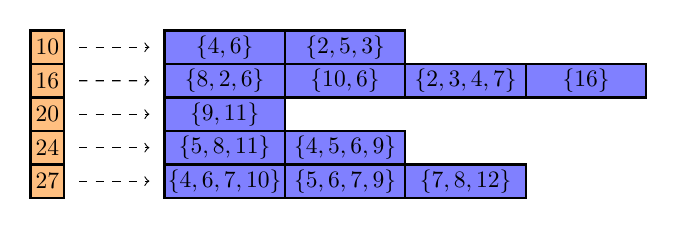
\begin{tikzpicture}
[
  scale=0.85,
  transform shape,
	key/.style={thick,fill=orange!50},
	value/.style={thick,fill=blue!50},
	other/.style={fill=yellow!10,dashed}
]

\draw (2,2) rectangle +(0.5, .5) [key] node[midway] {\textit{$10$}};
\node (10) at(2.6,2.25) {};

\draw (2,1.5) rectangle +(0.5, .5) [key] node[midway] {\textit{$16$}};
\node (16) at(2.6,1.75) {};

\draw (2,1) rectangle +(0.5, .5) [key] node[midway] {\textit{$20$}};
\node (20) at(2.6,1.25) {};

\draw (2,0.5) rectangle +(0.5, .5) [key] node[midway] {\textit{$24$}};
\node (24) at(2.6,0.75) {};

\draw (2,0) rectangle +(0.5, .5) [key] node[midway] {\textit{$27$}};
\node (27) at(2.6,0.25) {};


\node (10s) at(3.9,2.25) {};
\draw (4,2) rectangle +(1.8, .5) [value] node[midway] {\textit{$\{4,6\}$}};
\draw (5.8,2) rectangle +(1.8, .5) [value] node[midway] {\textit{$\{2,5,3\}$}};

\node (16s) at(3.9,1.75) {};
\draw (4,1.5) rectangle +(1.8, .5) [value] node[midway] {\textit{$\{8,2,6\}$}};
\draw (5.8,1.5) rectangle +(1.8, .5) [value] node[midway] {\textit{$\{10,6\}$}};
\draw (7.6,1.5) rectangle +(1.8, .5) [value] node[midway] {\textit{$\{2,3,4,7\}$}};
\draw (9.4,1.5) rectangle +(1.8, .5) [value] node[midway] {\textit{$\{16\}$}};

\node (20s) at(3.9,1.25) {};
\draw (4,1) rectangle +(1.8, .5) [value] node[midway] {\textit{$\{9,11\}$}};

\node (24s) at(3.9,0.75) {};
\draw (4,0.5) rectangle +(1.8, .5) [value] node[midway] {\textit{$\{5,8,11\}$}};
\draw (5.8,0.5) rectangle +(1.8, .5) [value] node[midway] {\textit{$\{4,5,6,9\}$}};

\node (27s) at(3.9,0.25) {};
\draw (4,0) rectangle +(1.8, .5) [value] node[midway] {\textit{$\{4,6,7,10\}$}};
\draw (5.8,0) rectangle +(1.8, .5) [value] node[midway] {\textit{$\{5,6,7,9\}$}};
\draw (7.6,0) rectangle +(1.8, .5) [value] node[midway] {\textit{$\{7,8,12\}$}};

\draw [->,thin, dashed] (10) -- (10s);
\draw [->,thin, dashed] (16) -- (16s);
\draw [->,thin, dashed] (20) -- (20s);
\draw [->,thin, dashed] (24) -- (24s);
\draw [->,thin, dashed] (27) -- (27s);

\end{tikzpicture}

  \caption{This figure shows the macrostate cache based on a hash table where key is the sum of a macrostate and a value is a list of the macrostates.}
  \label{figMacroCache}
\end{center}
\end{figure}

\section{Implementation of Antichain Algorithm}
The implementation of the algorithm for checking language inclusion of NFA using antichains has been done by algorithm described in section 
\ref{sectionAntichain}.  There were used data structures for representing antichains (classes \emph{Antichain2Cv2} and \emph{Antichain1c}) which
were implemented for the modules for the tree automata. 

The improvement of the antichain algorithm by using simulation is implemented too. 
This is done by parameterization of class for checking inclusion, where one of the given parameters is a relation which is simulation or identity (default).

Some optimization of this algorithm has been done during implementation and will be described in following subsections. For further subsections we suppose
checking inclusion between a NFA $\mathcal{A}$ and a NFA $\mathcal{B}$.

\subsection{Ordering of Antichain}
The antichain algorithms keeps only the minimal set of the visited product states with respect to ordering given by $(r,R)\sqsubseteq (p,P)$
iff $p=r \wedge R \subseteq P$. The ordering $p\preceq r \wedge R\preceq^{\forall\exists}P$ is used for the optimization by simulation.
Comparing $(r,R)$ and $(p,P)$ was implemented by one parameterized function for both orderings what is possible because $p=r$ is special case of $p\preceq r$ 
and the same holds for $R \subseteq P$ and $R\preceq^{\forall\exists}P$. But this implementation has shown as inefficient and the special implementation of
this function for each ordering alone should be more efficient because $R\subseteq P$ could be decided 
without comparing both sets element by element when size of the macrostate $R$ is greater then size of the macrostate $P$ while in case of
$R\preceq^{\forall\exists}P$ one element of macrostate $P$ could simulate all elements of $R$ so the size comparison is impossible.
The ordering using simulation also needs to iterate through all visited product states to find all the elements $p$ such that $p\preceq r$ what 
is not necessary in the case of basic version where is checked just $p=r$.

On the other side, the other optimization of simulation is based on the fact that if there is $p' \in P$ such that $p \preceq p'$ 
it is not needed to kept and further processed the product state $(p,P)$. When one parameterized function is used for both versions of the algorithm, it 
causes unnecessary slowing down because the condition is always false in case of basic version of the algorithm. 
Although this optimization has not been already implemented, we suppose that the separation of the functions will be also 
efficiently used in this case.

\subsection{Using Macrostate Cache}
The antichain algorithm often checks whether $R \subseteq P$ or $R\preceq^{\forall\exists}P$ which can be both quite expansive operations and it can be
efficient to store the results of these operations. Macrostate cache has been applied for this purpose so all used macrostates (such as $R$ or $P$) 
are stored in this cache. Then it is possible to work just with pointers to the cache and what helps efficiently store relation between $R$ and $P$. For example, 
the pointer to $R$ is mapped to the pointer to $P$ by a hash table when there is relation between $R$ and $P$. There is also a hash table that maps
the pointer to macrostate $R$ to pointers to all macrostates which are not in relation with $R$.

\subsection{Ordered Antichain}
For checking inclusion of tree automata has not been used standard antichain, but for storing product states $(p,P)$ which should be further processed
is used ordered antichain \cite{libvata} which prefers processing the elements with smaller size of macrostate $P$ first. This optimization leads to reduction
of produced states. The optimization has been implemented 
also for checking language inclusion of NFA and it reduces the number of produced product states too what brings the better performance.

%No further optimization for antichain algorithm are used so it is not as efficient as the algorithm based on bisimulation up to congruence and not even as the 
%tree version of this algorithm which is highly optimized. The suggestions for some optimization are given in another section \ref{Conclusion}.

\section{Translation of an NFA to LTS}
Before computing simulation relation over an NFA it is necessary to convert the NFA to labeled transition system (LTS), sort the states of the NFA to
two or three partitions (final, non-final and class representing start state) and initialize the simulation relation. This is done by algorithm where 
all transitions of NFA are converted to the LTS and at the same time each of the processed states is sorted to the partitions in according if
the state is final or not. If all states are final, there will be created only one partition in this part of the algorithm otherwise two partitions will
be created. After all transitions are processed, there is added another one partition which represents start states. Then the simulation relation is initialized
by the rules that each final state simulates other final state and each non-final simulates other non-final. The non-final one does not simulate final one, but 
final one simulates non-final one.

The created partitions, LTS and initialized simulation is given to the algorithm for computing the whole simulation. 

\section{Implementation of Bisimulation up to Congruence Algorithm}
\label{sectionCongrImpl}
The algorithm for checking inclusion of the languages of NFA is described in its own section \ref{sectionCongr}. For computation of a congruence closure, 
what is crucial part of the approach, was used an algorithm based on the rewriting rules (described \ref{subsectionCongr}). 
This algorithm was implemented generally for checking equivalence of NFA and its optimized version for checking inclusion was implemented too 
because the main goal of this work is to achieve the best performance of the inclusion checking. In this section will be described some implementation
optimization of the algorithm. For this section let think two NFA $\mathcal{A}=(Q_\mathcal{A},\Sigma,\delta_\mathcal{A},I_\mathcal{A},F_\mathcal{A})$ and
$\mathcal{B}=(Q_\mathcal{B},\Sigma,\delta_\mathcal{B},I_\mathcal{B},F_\mathcal{B})$.


\subsection{Exploring Product NFA}
Exploring of a product NFA $\mathcal{A}\times\mathcal{B}$ during checking inclusion between the languages of $\mathcal{A}$ and $\mathcal{B}$ could be done by 
the \emph{breadth-first search} \cite{taocp} algorithm or the \emph{depth-first search} \cite{taocp} algorithm what
determines order in which the states of the product NFA are explored. Usage of one or another algorithm can effect the number of states that are processed. 
Difference between this two approaches is in usage of a data structure for storing of the newly generated states of $\mathcal{A}\times\mathcal{B}$.
If the used data structure is list then breadth-first search is applied and if the used data structure is stack then 
depth-first search is applied.

The VATA library module for NFA currently supports only the breadth-first search algorithm. This approach has not been chosen for any special reason or superiority
but has evolved during the implementation because the antichain algorithm uses for storing of 
the newly generated states also list what leads to the implementation of breadth-first search.


\subsection{Using Macrostate cache}
When one checks inclusion (or equivalence) of languages of NFA $\mathcal{A}$ and $\mathcal{B}$ there are generated states states of product NFA $\mathcal{A}
\times \mathcal{B}$ which are pairs $(X,Y)$ where $X$ is macrostate of states of $\mathcal{A}$ and $Y$ is macrostate of states of $\mathcal{B}$. $X$ and $Y$
are stored to macrostates cache and it is further worked only with pointers to this macrostates in cache.

The original algorithm does not control if the newly generated state $(X,Y)$ has not already been visited and always checks if $(X,Y)$ is in
congruence closure of relation of the visited states $R$  what is
computationally demanding operation. Thanks to the working just with pointers to macrostates is easy to check whether the new state is already in a set of 
visited states without computing the congruence closure. It is done by hash table which maps pointer of a macrostate $Y$ to list of all
pointers to macrostates $X$ such that $(X,Y)\in R$. Then it is easy to check whether a newly generated state has not already been processed. 

This technique reduces the number of the states of $\mathcal{A}\times\mathcal{B}$ for which is necessary to compute congruence closure what helps improvement in
the performance of the whole algorithm.

\subsection{Computing Congruence Closure for Equivalence Checking}
The computation of the congruence closure of the visited states of an NFA $\mathcal{A}\times\mathcal{B}$ for equivalence checking using rewriting
rules as it was described in section \ref{subsectionCongr} is computationally demanding operation, 
so there were implemented an optimization to enhance the performance of the algorithm.

The optimization is based on the observing that when the normal form of macrostates $X$ and $Y$ for some relation $R$ are derived to find out if holds that
$(X,Y)\in c(R)$ it is not necessary to use all possible rewriting rules of $R$ and add as much states as possible to the normal form
of macrostate. It is possible to stop derivation of
$X{\downarrow_R}$ and $Y{\downarrow_R}$ when these sets are equal and it is also not necessary to achieve the equality $X{\downarrow_R}$ and $Y{\downarrow_R}$ by
applying the same rules, not even by the same number of rules. 
This fact makes possible to control $X{\downarrow_R} = Y{\downarrow_R}$ on the fly and not only after the whole derivation.

This simplification leads to the implementation optimization, which is based on creating of $X{\downarrow_R}$ by applying all possible rewriting rules
so it has as much states as possible. 
When a rule is applied during the derivation of $X{\downarrow_R}$ it is mapped in a hash table to 
the form of $X{\downarrow_R}$ after application of the rule.
Then $Y{\downarrow_R}$ is derived gradually and after each step is checked if the current form of $Y{\downarrow_R}$ is not same as any of the forms of
$X{\downarrow_R}$ which has been reached during its derivation. But comparing $Y{\downarrow_R}$ after each step to all forms of $X{\downarrow_R}$ is not efficient
and it slows down the algorithm instead of improving it. This leads to implementation where the form of $Y{\downarrow_R}$ after applying of a rewriting rule 
is compared to the form of $X{\downarrow_R}$ after the usage of the same rule. 
The second approach is not maybe so efficient because it is not detect if $X{\downarrow_R}=Y{\downarrow_R}$ as early as the first one but this disadvantage is
compensated by lesser comparison of $X{\downarrow_R}$ and $Y{\downarrow_R}$.

\subsection{Computing Congruence Closure for Inclusion Checking}
In section \ref{congrOpt} was described optimization that can be used when one uses the algorithm based on bisimulation up to congruence for checking 
the language inclusion. The optimization is based on the fact that inclusion checking is done by checking equivalence $\mathcal{A}\cup\mathcal{B}=\mathcal{B}$,
so for a state $(X,Y)$ holds $(X,Y)\in c(R)$ iff $X\subseteq Y{\downarrow_R}$ for a relation $R$ of visited states. 
This optimization was implemented in the VATA library module for NFA to achieve the best performance in checking language inclusion.

This optimization is further enhanced by the following implementation's improvements. Once there is checked a generated product state $(X,Y)$ and the normal form 
$Y{\downarrow_R}$ is computed it could be efficient to store all rewriting rules that was used during the computation because otherwise there can be
generated another product state with $Y$ in, e.g. $(Z,Y)$ and the whole computation of $Y{\downarrow_R}$ has to be done again. 

At the same time a rewriting rules can be used only in one direction ($Y\rightarrow X\cup Y$) for a $(X,Y)\in R$. So when there is checked
if a newly generated product state $(P,Q)$ is in a congruence closure of $R$ it is needed just to check if $Y \subseteq Q$ to apply 
the rewriting rule $Y\rightarrow X\cup Y$. If the rewriting rule is applied, macrostate $X$ is added to $Q{\downarrow_R}$. 
Once the rewriting rule is possible to apply we know that it is possible to apply all elements of $R$ containing $Y$ 
so it is efficient to store that $Y\subseteq Q$.

This principle of storing applicable rules is implemented by a hash table where a pointer to a macrostate $Q$ is mapped to
a list of pointers to the macrostates where each of this macrostates $Y$ enables to use all of the elements of relation $R$ containing $Y$ 
for computation of $Q{\downarrow_R}$.
Notice that is not able to store elements of $R$ which rewriting rule is not applicable because there are added gradually
new elements to $R$ and after applying of a new rewriting rule can be usable also rule which has not been usable last time.%Preformulovat

During the experimental evaluation was found that this optimization is not as useful as it was expected because it does not happen very often that the one
macrostate of NFA $\mathcal{B}$ (e.g. macrostate $Q$) is in the two different states of a product NFA $\mathcal{A}\cup\mathcal{B}\times\mathcal{B}$ (e.g., $(P,Q)$
and $(O,Q)$ where $P$ and $O$ are macrostates of $\mathcal{A}\cup\mathcal{B}$) and can slow down the algorithm because of the overhead given by checking
if a normal form $Q{\downarrow_R}$ has not already been computed, so it was implemented a special function for computing normal form of a visited macrostate 
and special function for computing normal forms of macrostates which has not been already explored. 

\chapter{Experimental Evaluation}
\label{eval}
This chapter is about the experimental evaluation of the algorithms for checking inclusion based on antichains and on the bisimulation up to congruence. 

For both of the evaluations were used NFA for model checking provided by Dr. Lukáš Holík\footnote{
Automata can be found on the web page: \url{http://www.fit.vutbr.cz/~holik/pub/ARMCautomata.tar.gz}}.  
The evaluation was done on the set of about 40 000 of pairs of NFA. 

The tests were performed on the server \emph{merlin.fit.vutbr.cz} with CentOS 64bit Linux, 2$\times$ AMD Opteron (2,5 GHz, 4 cores, 12 MB cache) and 8 GB Ram.

\section{Evaluation of Algorithm Based on Antichains}
The implementation of the antichain algorithm is compared to the VATA library implementation of the antichain algorithm for tree automata. The tree automata's
algorithms for checking language inclusion was tested in explicit encoding using upward direction and also downward direction. 
Timeout of computation was set to five seconds.

The comparison with the inclusion checking algorithm for tree automata in upward direction is given on the figure \ref{fig:figPlotAc} where the whole data
set is on the left plot and the right plot is focused. As it is written down in the table \ref{tabAc} the new implementation for NFA was faster in 98\% of the
test cases and in these cases was averagely two times faster. The tree automata's algorithm is faster only in two cases but in these cases is faster sixteen times.
This acceleration of the tree automata's algorithm is some cases is not yet analyzed and could be object of further development.

\begin{figure}[bt]
\begin{center}
\includegraphics[scale=0.3]{fig/plot_aac_zprava.png}
\includegraphics[scale=0.3]{fig/plot_aac_step_zprava.png}
\caption{The comparison of VATA library implementation of antichain algorithm for tree automata in upward direction
    with VATA library implementation of the antichain algorithm for NFA.}
\label{fig:figPlotAac}
\end{center}
\end{figure}

The comparison of the new implementation of the algorithm for NFA with implementation for tree automata in downward direction using optimized cache
is given on the figure 
\ref{fig:figPlotAc} where the left plot again shows the whole data set and the right one shows focus on the time interval where the most of tests belong.
The algorithm for NFA beats the tree automata's algorithm in the most cases (about 93\%) and is about 211 times faster (all data are in table \ref{tabAc}).

\begin{table}[bt]
\begin{center}
\parbox{.45\linewidth}{
  \begin{tabular}[scale=0.3]{ | l | r | r |}
   \hline
    & \textbf{AC UP} & \textbf{AC NFA} \\ \hline \hline
    winner & $2\%$ & $98\%$ \\ \hline
    faster & $15.91\times$ & $2.65\times$ \\ \hline
   \end{tabular}
}
   \parbox{.45\linewidth}{
  \begin{tabular}{ | l | r | r |}
   \hline
    & \textbf{AC DOWN} & \textbf{AC NFA} \\ \hline \hline
    winner & $7\%$ & $93\%$ \\ \hline
    faster & $10.78\times$ & $211.42\times$ \\ \hline
   \end{tabular}
   }
   \caption{The left table shows comparison of VATA library for tree automata with checking inclusion in upward direction using the antichain algorithm with
       implementation of the antichain algorithm for NFA and
   the right table shows the same comparison but with for the downward direction version of the antichain tree automata's algorithm optimized
   by cache.}
   \label{tabAac}
\end{center}
\end{table}



\begin{figure}[bt]
\begin{center}
\includegraphics[scale=0.3]{fig/plot_aca_zprava.png}
\includegraphics[scale=0.3]{fig/plot_aca_step_zprava.png}
\caption{The figure shows
 comparison of VATA library implementation of the antichain algorithm for tree automata in downward direction using cache optimization 
 with VATA library implementation of the antichain algorithm for NFA.}
\label{fig:figPlotAca}
\end{center}
\end{figure}

\section{Evaluation of Algorithm Based on Bisimulation up to Congruence}
The evaluation of the algorithm based on bisimulation up to congruence was done by implementation which includes all optimization described in section 
\ref{sectionCongrImpl}. There are provided two comparison, the first one is with original OCaml implementation of this algorithm and the second one is with
VATA library module for tree automata.

\subsection{Comparison with OCaml Implementation}
The algorithm based on bisimulation up to congruence was implemented 
\footnote{The implementation can be found here: \url{http://perso.ens-lyon.fr/damien.pous/hknt/}} 
in \emph{OCaml} language (object-oriented implementation of Caml language). 
This implementation provides checking of the equivalence
and the inclusion of languages of NFA and also inclusion. It is also possible to use breadth-first search or depth-first search algorithm for searching 
product NFA and it is possible to use a simulation for improvement of performance of the algorithm.

For evaluation purposes was OCaml implementation run with breadth-first search (which is the only one currently implemented by VATA library), without
simulation (which is not currently not provided by VATA library) and in the version for inclusion checking.

The comparison of the VATA library implementation and OCaml implementation can be seen on the figure \ref{fig:figGraphOCaml}. 
The plot shows the relation between time needed to check language inclusion and number of the states of the input NFA.
The left plot shows the measurements on the whole data set and it is possible to see that the VATA library is especially faster for input automata with a lot
of states. The right plot on the figure \ref{fig:figGraphOCaml} is focused to the time interval where are the most of the measurements belong and 
shows that in some cases is OCaml implementation faster. In these cases only a few states were explored to 
check the language inclusion and the VATA library was slower due the overhead caused by its richer data structures (like macrostate cache). The plot also shows
how time needed to check inclusion grows exponentially with number of states of NFA but 
the growth of amount of time is much faster in case of OCaml implementation.

The VATA library was faster in $92.5\%$ of tested cases and in these cases were faster about 65 times, particular data are in the table \ref{tabOcaml}.

\begin{figure}[bt]
\begin{center}
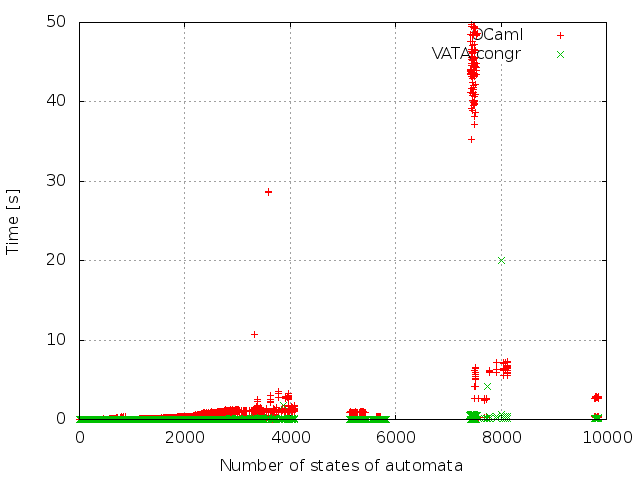
\includegraphics[scale=0.3]{fig/plot_hkc_zprava.png}
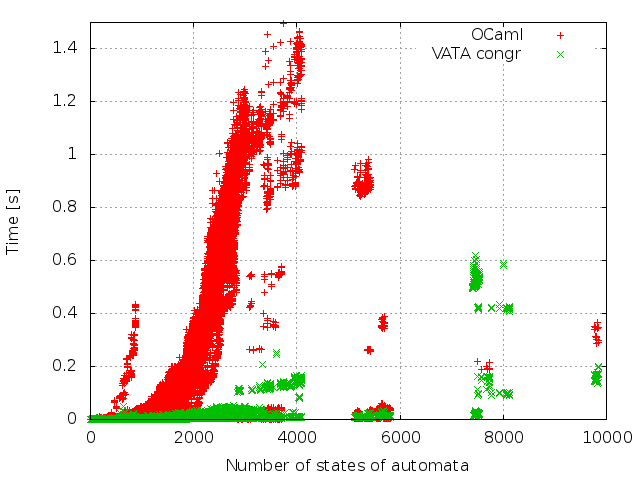
\includegraphics[scale=0.3]{fig/plot_hkc_step_zprava.png}
\caption{
Comparison of OCaml implementation of a congruence algorithm and VATA library implementation of the algorithm.}
\label{fig:figGraphOCaml}
\end{center}
\end{figure}

\begin{center}
\begin{table}[tb]
\begin{center}
  \begin{tabular}{ | l | r | r |}
   \hline
    & \textbf{OCaml} & \textbf{VATA} \\ \hline \hline
    winner & $7.5\%$ & $92.5\%$ \\ \hline
    faster & $6.43\times$ & $64.29\times$ \\ \hline
   \end{tabular}
   \caption{Table gives summarizing of the evaluation of comparing of OCaml implementation of a congruence algorithm and VATA library implementation 
     of the algorithm.}
   \label{tabOcaml}
\end{center}
\end{table}
\end{center}

\subsection{Comparison with Tree Automata Implementation of VATA Library}
It was also made evaluation which compares the VATA library for checking language inclusion of tree automata based on antichain algorithm. The 
VATA library for tree automata was used with explicit encoding and inclusion was checked in upward and also downward direction. For downward direction was used
optimization based on a cache. The timeout for checking inclusion was set to 5 seconds.

The result of comparison of the checking language inclusion using bisimulation up to congruence for NFA and antichains for tree automata 
is given on the figures \ref{fig:figPlotAc} and \ref{fig:figPlotCa}, particular on the left plot in these figures. The plot shows number of states of the input
automaton and time needed to check the inclusion. The new implementation for finite automata is faster in the
most (about $95\%$) cases but is only about two times faster then the algorithm for upward direction. 
Checking language inclusion using downward direction is much slower than 
the congruence algorithm which is faster in $94\%$ of cases  and is faster for one hundred and sixty times. The particular data about speed up 
which brings implementation for NFA is given in table \ref{tabAc}.

The figures \ref{fig:figPlotAc} and \ref{fig:figPlotCa} also show
focus to a time interval where the most measurements belong. The figures show that VATA library for tree automata was
also faster in some cases, what is caused by the fact the both approaches (antichain and bisimulation up to congruence) uses different attributes of relation
of set of states that is necessary to check to verify if language inclusion holds.

\begin{figure}[bt]
\begin{center}
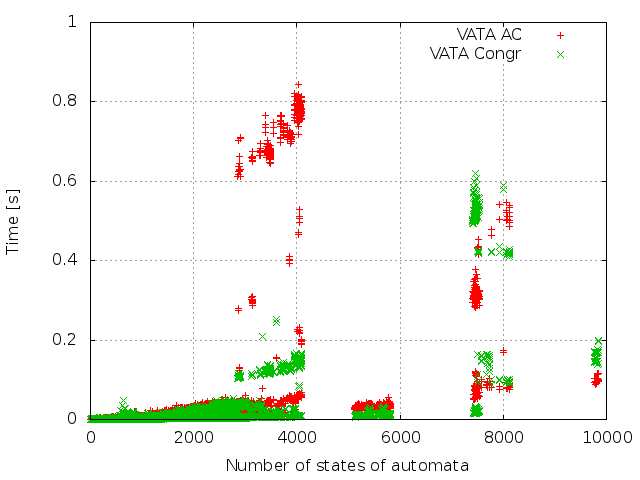
\includegraphics[scale=0.3]{fig/plot_ac_zprava.png}
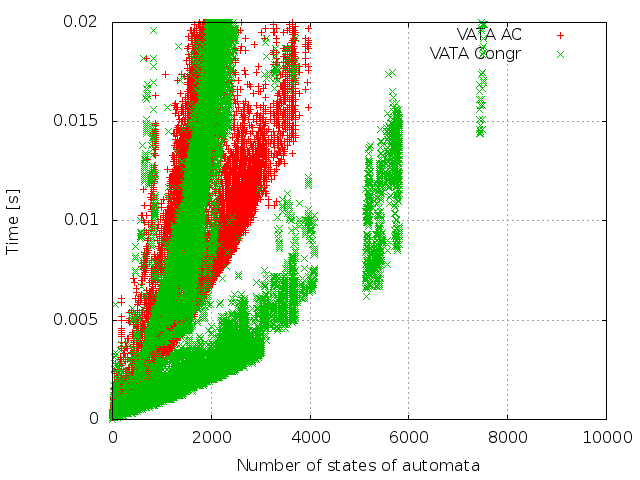
\includegraphics[scale=0.3]{fig/plot_ac_step_zprava.png}
\caption{The comparison of VATA library implementation of the antichain algorithm for tree automata in upward direction
    with VATA library implementation of the congruence algorithm for NFA.}
\label{fig:figPlotAc}
\end{center}
\end{figure}

\begin{table}[bt]
\begin{center}
\parbox{.45\linewidth}{
  \begin{tabular}[scale=0.3]{ | l | r | r |}
   \hline
    & \textbf{AC UP} & \textbf{CONGR} \\ \hline \hline
    winner & $5\%$ & $95\%$ \\ \hline
    faster & $1.27\times$ & $2.34\times$ \\ \hline
   \end{tabular}
}
   \parbox{.45\linewidth}{
  \begin{tabular}{ | l | r | r |}
   \hline
    & \textbf{AC DOWN} & \textbf{CONGR} \\ \hline \hline
    winner & $6\%$ & $94\%$ \\ \hline
    faster & $1.90\times$ & $160.34\times$ \\ \hline
   \end{tabular}
   }
   \caption{The left table shows comparison of VATA library for tree automata with checking inclusion upward with antichain algorithm with
       implementation of the algorithm based on bisimulation up to congruence and
   the right table shows the same comparison but with for the downward version of the antichain algorithm optimized by cache.}
   \label{tabAc}
\end{center}
\end{table}

\begin{figure}[t]
\begin{center}
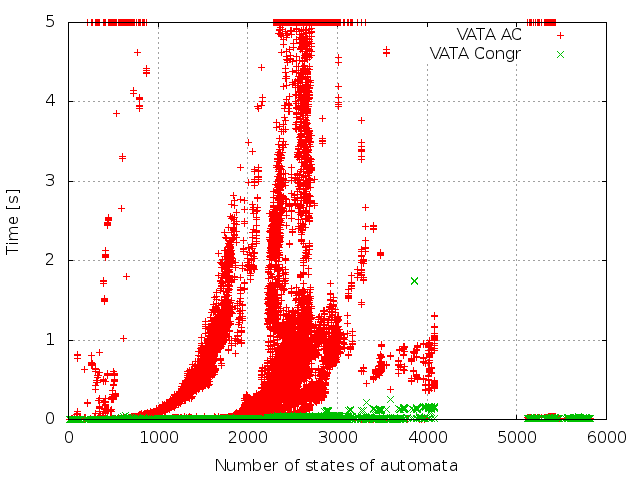
\includegraphics[scale=0.3]{fig/plot_ca_zprava.png}
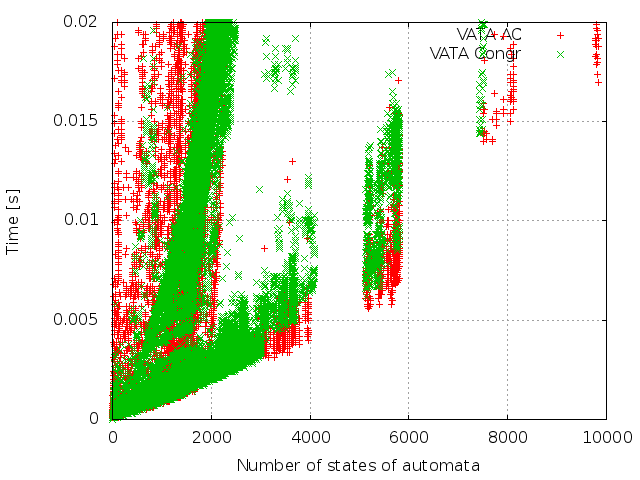
\includegraphics[scale=0.3]{fig/plot_ca_step_zprava.png}
\caption{The figure shows
 comparison of VATA library implementation of the antichain algorithm for tree automata in downward direction using cache optimization 
 with VATA library implementation of the congruence algorithm for NFA.}
\label{fig:figPlotCa}
\end{center}
\end{figure}

\section{Comparison of the algorithm for NFA}
Finally, the both newly implemented algorithms for NFA, the one based on the antichains and the one based on bisimulation up to congruence, will be compared.
The both algorithms were used in their optimized versions.
The comparison is shown on the figure \ref{fig:figPlotNFA}.
As you can see, the results of the evaluations of both algorithms are very similar and the differences in the performance of
them are very small. 
The results are summarized in the table \ref{tabNFA}. The antichain algorithm beats the congruence algorithm in 75\% of
tested cases. On the other side, the congruence algorithm is nearly four times faster in its winning cases than the antichain algorithm which is
only 1.5 times faster in its winning cases. 
It is important notice that the results are dependent on the chosen test set because the both uses different attributes
of the set of explored states of NFA during language inclusion checking.

\begin{figure}[bt]
\begin{center}
\includegraphics[scale=0.3]{fig/plot_nfa_ac_zprava.png}
\includegraphics[scale=0.3]{fig/plot_nfa_congr_zprava.png}
\caption{The comparison of VATA library implementation of the antichain algorithm for NFA (the left plot)
    with VATA library implementation of the congruence algorithm for NFA (the right plot).}
\label{fig:figPlotNFA}
\end{center}
\end{figure}

\begin{table}[bt]
\begin{center}
\parbox{.45\linewidth}{
  \begin{tabular}[scale=0.3]{ | l | r | r |}
   \hline
    & \textbf{AC} & \textbf{CONGR} \\ \hline \hline
    winner & $76\%$ & $24\%$ \\ \hline
    faster & $1.58\times$ & $3.74\times$ \\ \hline
   \end{tabular}
}
   \caption{Table shows result of comparison of the congruence algorithm and the antichain algorithm for NFA.}
   \label{tabNFA}
\end{center}
\end{table}

\chapter{Conclusion}
\label{concl}
The main goal of this thesis is to create an extension of the VATA library for the nondeterministic finite automata 
which are often used in the formal verification (e.g., model checking of safety temporal properties or 
abstract regular model checking) what is the branch of computer science which is the library focused on. The extension of the library is supporting
basic operations like union, intersection, removing useless or unreachable states and etc., but the main aim of this work is to provide
efficient implementation of the state-of-the-art algorithms for checking language inclusion of nondeterministic finite automata.

The new extension of VATA library uses the explicit encoding for representation of the finite automata. 
The data structures for the explicit encoding has been designed
and implemented by modification and optimization of the data structures for the tree automata. The original VATA library has been analyzed to be able to determine
which modules can be reused for a new extension and also to be able efficiently integrate the new extension.

To achieve the best performance for language inclusion checking are used the state-of-the-art algorithms, based on so-called antichains and so-called bisimulation
up to congruence. The antichains algorithms is implemented in its default version and also optimized version which uses simulation of a finite automaton. 
The bisimulation up to congruence algorithm is implemented in its general version (for checking equivalence of finite automata) and also in
version specialized to checking inclusion what brings better performance. The other improvement of this algorithm is realized by implementation's optimization.

For proving contribution of this work has been performed evaluation which compares the performance of our implementation of language
inclusion checking to the other implementations. 
Our implementation beats the other tested implementation in over 90\% of the tested cases. It faster about 100 times then the OCaml implementation of the
algorithm for congruence closure and 2 times then the tree automata's algorithm.

The analysis of the cases where the tree automata's algorithm for language inclusion checking significantly 
beats the implementation specialized on NFA could be done for further optimization of the implementation. 
For the bisimulation up to congruence algorithm is possible to implement version of the algorithm 
which uses simulation for pruning out some other states which are not necessary to explore. The simulation is yet implemented for antichain algorithm for NFA but
it has not been evaluated and optimized what can bring another improvement of performance. The full integration of the new extension of the
VATA library could be done by application of it in the fields where the implementation of VATA library for tree automata is used.
 % viz. obsah.tex

  % Pouzita literatura
  % ----------------------------------------------
\ifczech
  \bibliographystyle{czechiso}
\else 
  \bibliographystyle{plain}
%  \bibliographystyle{alpha}
\fi
  \begin{flushleft}
  \bibliography{literatura} % viz. literatura.bib
  \end{flushleft}
  \appendix
  
  \chapter{Storage Medium}
The storage medium contains the sources of the VATA library including the new extension for finite automata. It also contains electronic version of this the text
report.
%\chapter{Manual}
%\chapter{Konfigrační soubor}
%\chapter{RelaxNG Schéma konfiguračního soboru}
%\chapter{Plakat}

 % viz. prilohy.tex
\end{document}
